
The signal reconstruction efficiencies may differ for the individual $\PgU(nS)$ states reconstructed in the \pp and \PbPb data. 
These are expected to cancel to first order in the double ratio. 
In this section, these efficiencies and their residual differences are estimated, based on Monte Carlo simulation.
%
In particular, in order to estimate the corresponding corrections required for the double ratio, the reconstruction efficiency is calculated as a function of centrality for the \PgUa and \PgUb states. 


When referring to the ratios measured in the analysis, we use the notation specified in 
Equations~\ref{eqn:def:r23}, \ref{eqn:def:r2}, \ref{eqn:x23:def}, and \ref{eqn:x2:def} in Sec.~\ref{sec:dooubleratio} and Eq.~\ref{eq:raa} in Sec.~\ref{sec:absolute}.  


\subsection{Monte Carlo estimations}
\label{sec:eff:mc}

In order to make the comparison for the reconstruction (including online and offline selections) efficiency for the \PgUa and \PgUb in \PbPb and \pp collisions, Monte Carlo events are used, where an \PgU is produced and decays via the \mumu channel. We use  $\varepsilon={N_{reco}}/{N_{gen}}$, where $N_{gen}$ is the number of events that fall within our acceptance conditions ($|\eta| < 2.4$, $p_{T} > 4 (3.5)$ for each of the muons),  and $N_{reco}$ is the number of dimuons that are reconstructed, match the trigger, pass the quality cuts presented in Section~\ref{sec:selection}, and fall within an invariant-mass window of $[9.0,10.0]$ for \PgUa and $[9.5,10.5]$ for $\PgUb$. Yields were estimated by counting and, alternatively, fitting the MC mass spectrum to account for backgrounds.  

Tables~\ref{Tab:RecEff4} and~\ref{Tab:RecEff35} show the reconstruction efficiencies of $\PgUa$ and $\PgUb$ in various centrality bins with two different single muon $\pt$ cuts. 
%An additional cut of dimuon vertex probability $> 5 \%$ with other single muon quality cuts is applied. %NOte: this is not additional, it is the new default! so no need to mention
It is observed, in \fig{fig:EffRatioCent_pt}, that the ratio of \PgUa and \PgUb efficiencies in \PbPb collisions are flat with respect to the centrality bins used in the analysis. 
%%%%%%%%%%%%%%%%%%%%%%%%%%%%%%%%%%%%%%%%%%
\begin{table}[h!]
\begin{center}
\caption{Reconstruction efficiency for $\PgUa$ and $\PgUb$ embedded in MB HYDJET sample. An acceptance cut of single muon $p_{T} > 4.0 \GeVc$ is applied for these values.} 
\label{Tab:RecEff4}
\begin{tabular}{c|c|c|c}
  \hline
&   Centrality              &$\PgUa$    &$\PgUb$  \\ %&$\PgUa$ pp    &$\PgUb$ pp \\ 
  \hline
\multirow{10}{*}{\PbPb} 
&   $[0-100\%]$            &$48.6\pm0.2\%$     &$49.3\pm0.2\%$ \\ 

&   $[0-5\%]$              &$46.6\pm0.6\%$     &$47.3\pm0.8\%$ \\
&   $[5-10\%]$             &$47.1\pm0.6\%$     &$48.0\pm0.8\%$ \\
&   $[10-20\%]$            &$49.2\pm0.5\%$     &$49.0\pm0.5\%$ \\
&   $[20-30\%]$            &$49.1\pm0.5\%$     &$50.2\pm0.5\%$ \\
&   $[30-40\%]$            &$51.0\pm0.4\%$     &$51.1\pm0.5\%$ \\
&   $[40-50\%]$            &$51.7\pm0.5\%$     &$51.5\pm0.5\%$ \\
&   $[50-100\%]$           &$51.6\pm0.3\%$     &$53.0\pm0.3\%$ \\
\cline{2-4}
&   $[50-60\%]$            &$51.1\pm0.4\%$     &$53.0\pm0.4\%$ \\
&   $[50-100\%]$           &$52.1\pm0.3\%$     &$53.0\pm0.3\%$ \\
\hline
\pp&  --                   &$48.7\pm0.1\%$     &$49.4\pm0.2\%$ \\
\hline 
\end{tabular}
\end{center}
\end{table}


\begin{table}[h!]
\begin{center}
\caption{Reconstruction efficiency for $\PgUa$ and $\PgUb$ embedded in MB HYDJET sample. An acceptance cut of single muon $p_{T} > 3.5$ GeV is applied for these values; the corresponding results for the nominal analysis selection are shown in Table~\ref{Tab:RecEff4}.} 
\vspace{1em}
\label{Tab:RecEff35}
\begin{tabular}{c|c|c|c}
  \hline
&   Centrality              &$\PgUa$    &$\PgUb$  \\
%&$\PgUa$ pp    &$\PgUb$ pp \\ 
\hline 
\multirow{7}{*}{\PbPb} 
   &   $[0-100\%]$            &$43.6\pm0.2\%$     &$44.8\pm0.2\%$  \\  
   
   &   $[0-5\%]$              &$41.8\pm0.5\%$     &$43.0\pm0.7\%$  \\
   &   $[5-10\%]$             &$42.1\pm0.5\%$     &$44.2\pm0.6\%$  \\
   &   $[10-20\%]$            &$44.1\pm0.4\%$     &$44.2\pm0.4\%$  \\
   &   $[20-30\%]$            &$44.4\pm0.4\%$     &$45.3\pm0.4\%$  \\
   &   $[30-40\%]$            &$45.4\pm0.4\%$     &$46.9\pm0.4\%$  \\
   &   $[40-50\%]$            &$46.0\pm0.4\%$     &$46.9\pm0.4\%$  \\
   &   $[50-60\%]$            &$46.4\pm0.2\%$     &$47.2\pm0.4\%$  \\
   &   $[60-100\%]$           &$46.9\pm0.2\%$     &$47.9\pm0.2\%$  \\    

\hline 
\pp&    --                    &$43.5\pm0.08\%$    &$44.6\pm0.2\%$  \\
\hline 
\end{tabular}
\end{center}
\end{table}


\begin{figure}[h!]
  \begin{center}
  
  %    \subfigure[$\pt^\mu > 3.5\GeVc$]{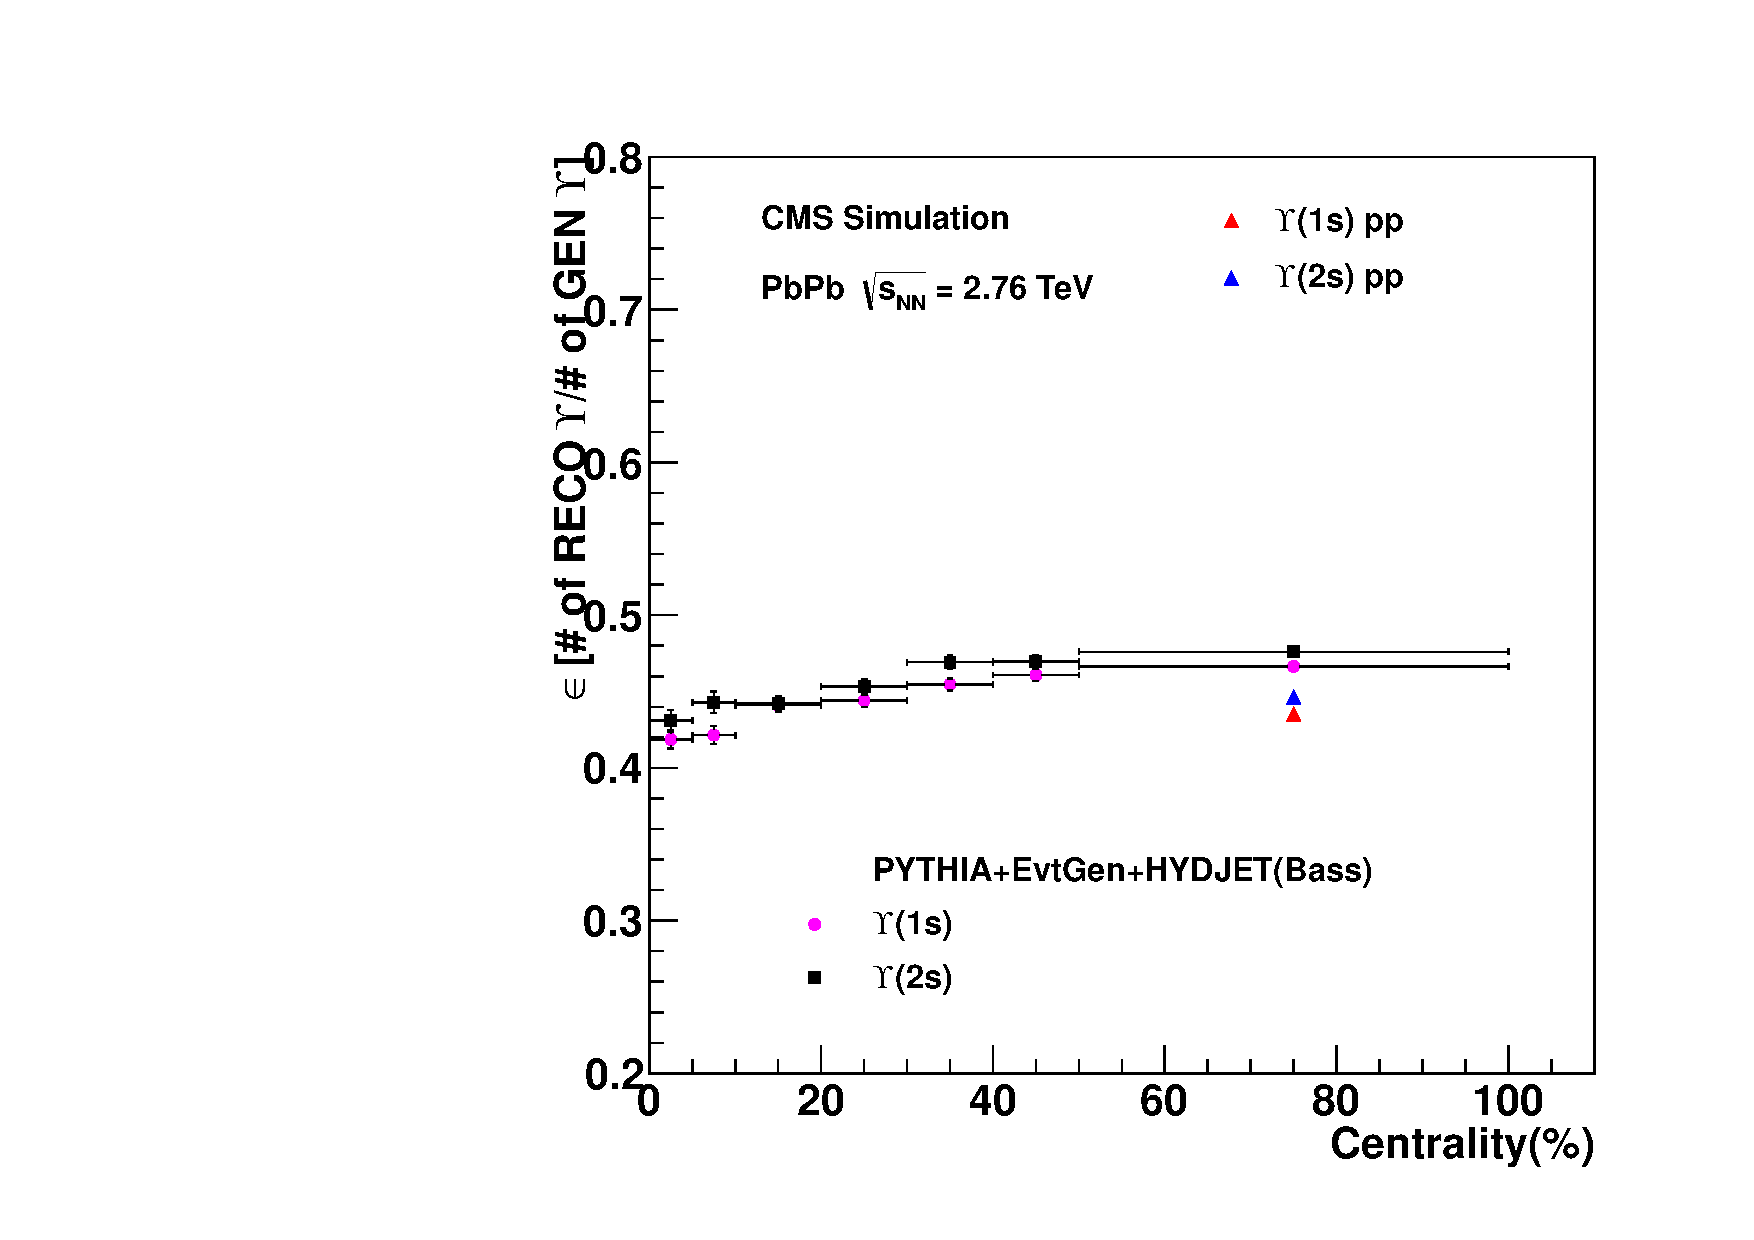
\includegraphics[angle=0,width=0.49\textwidth]{figures/efficiency/Ups_EffCent_pt35}}
   \subfigure[$\pt^\mu > 3.5\GeVc$]{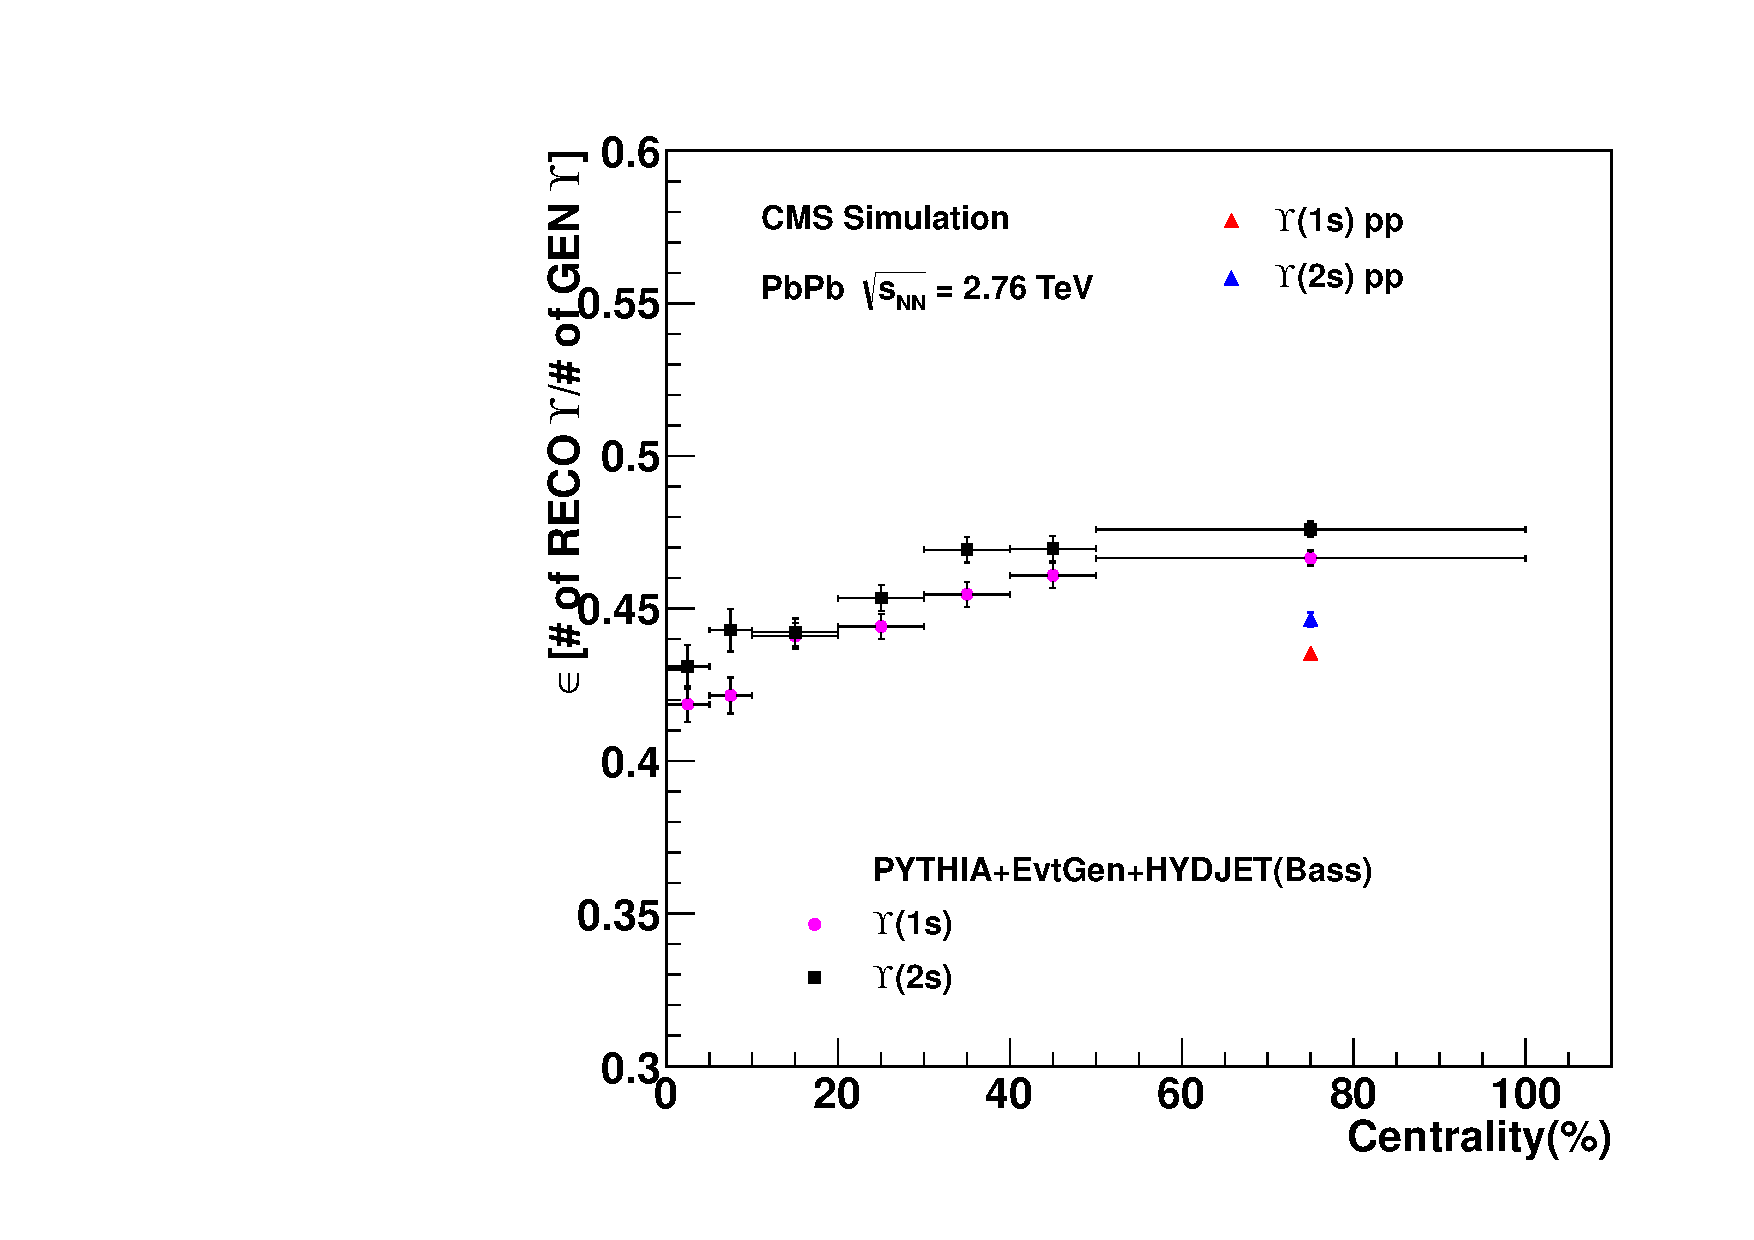
\includegraphics[angle=0,width=0.49\textwidth]{figures/efficiency/EffiCentPt35}}
   \subfigure[$\pt^\mu > 4\GeVc$]{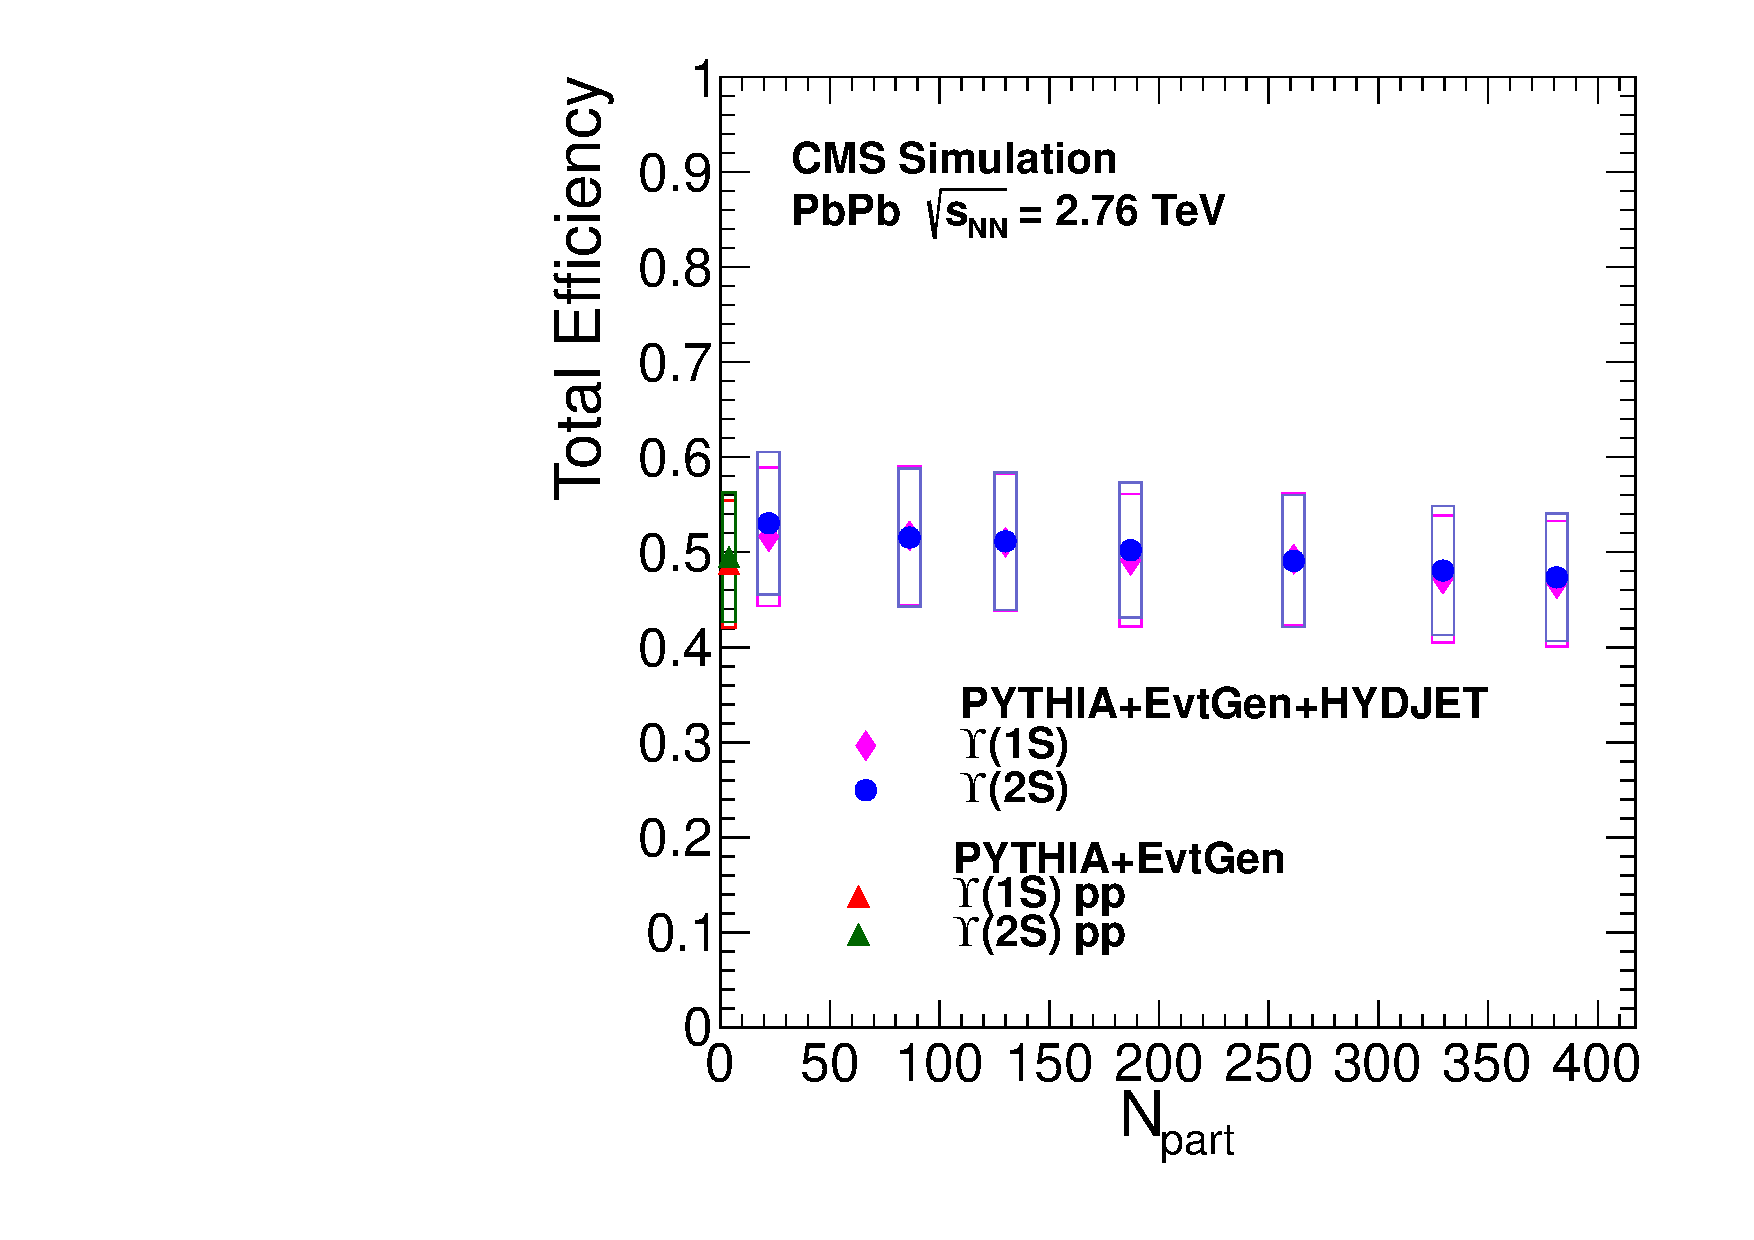
\includegraphics[angle=0,width=0.5\textwidth]{figures/efficiency/EffiCentPt40}}
   

   % \subfigure[$\pt^\mu > 4\GeVc$]{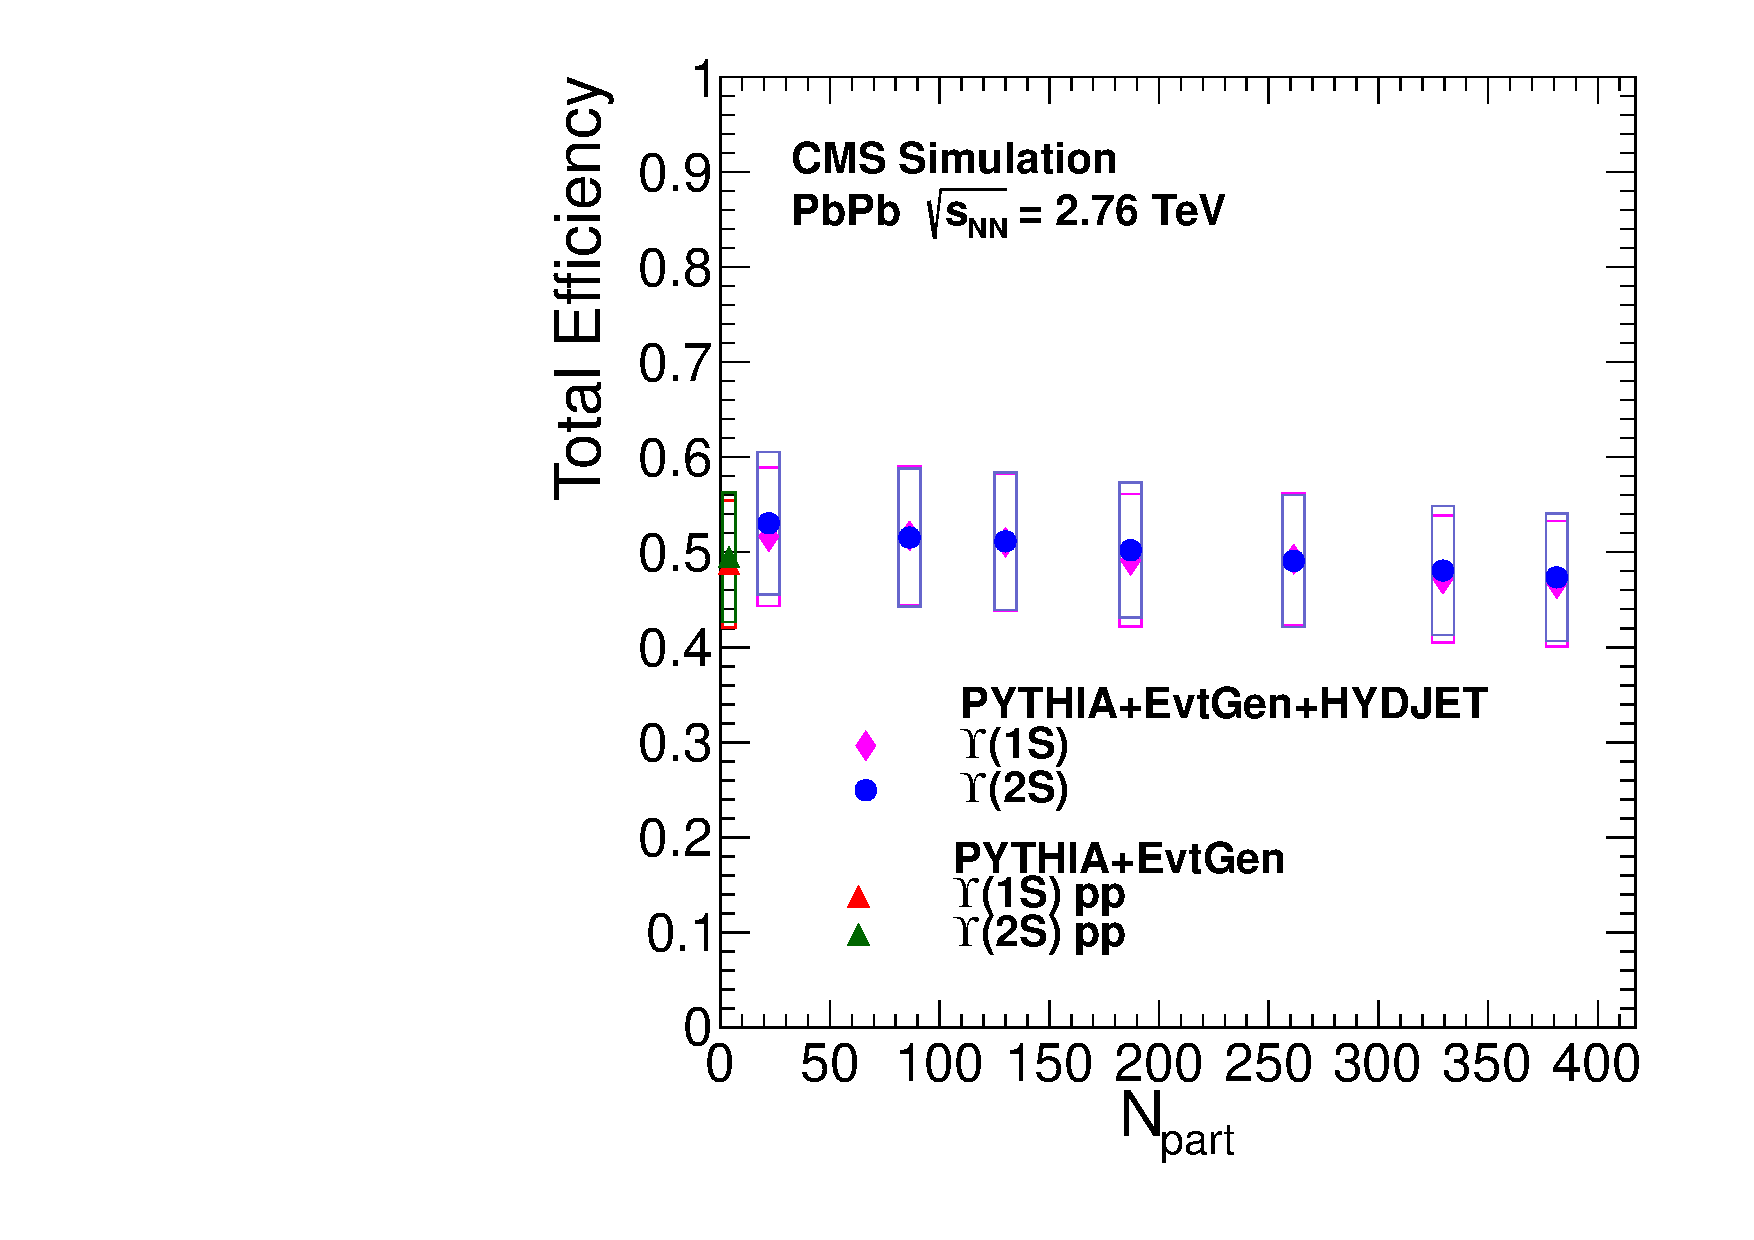
\includegraphics[angle=0,width=0.5\textwidth]{figures/efficiency/Ups_EffCent_pt4}}
    \caption{Total efficiency as a function of centrality, comparing \PbPb and \pp.}
    \label{fig:EffCent}
  \end{center}
\end{figure}


Figure~\ref{fig:EffCent} shows the centrality dependence of the ${\PgUa}$ and ${\PgUb}$ total efficiencies in \PbPb, compared with the same in \pp.
%
The efficiency, for either \PgUa\ or \PgUb\ in \PbPb, is shown to decrease as a function of the event centrality (being smallest for the highest multiplicity events, or lowest centrality percentile). This is expected, as the effect of larger tracking reconstruction inefficiencies for the higher track multiplicities which characterize the more central collisions. 
%
The slightly larger efficiency for \PgUb than \PgUa arises from the softer muon distribution from \PgUa decays, illustrated in \fig{fig:muon_properties_4_0}. 

\begin{figure}[h!]
  \begin{center}
    \subfigure[Total \PgUa efficiency. The red triangle indicates the \pp efficiency. ]{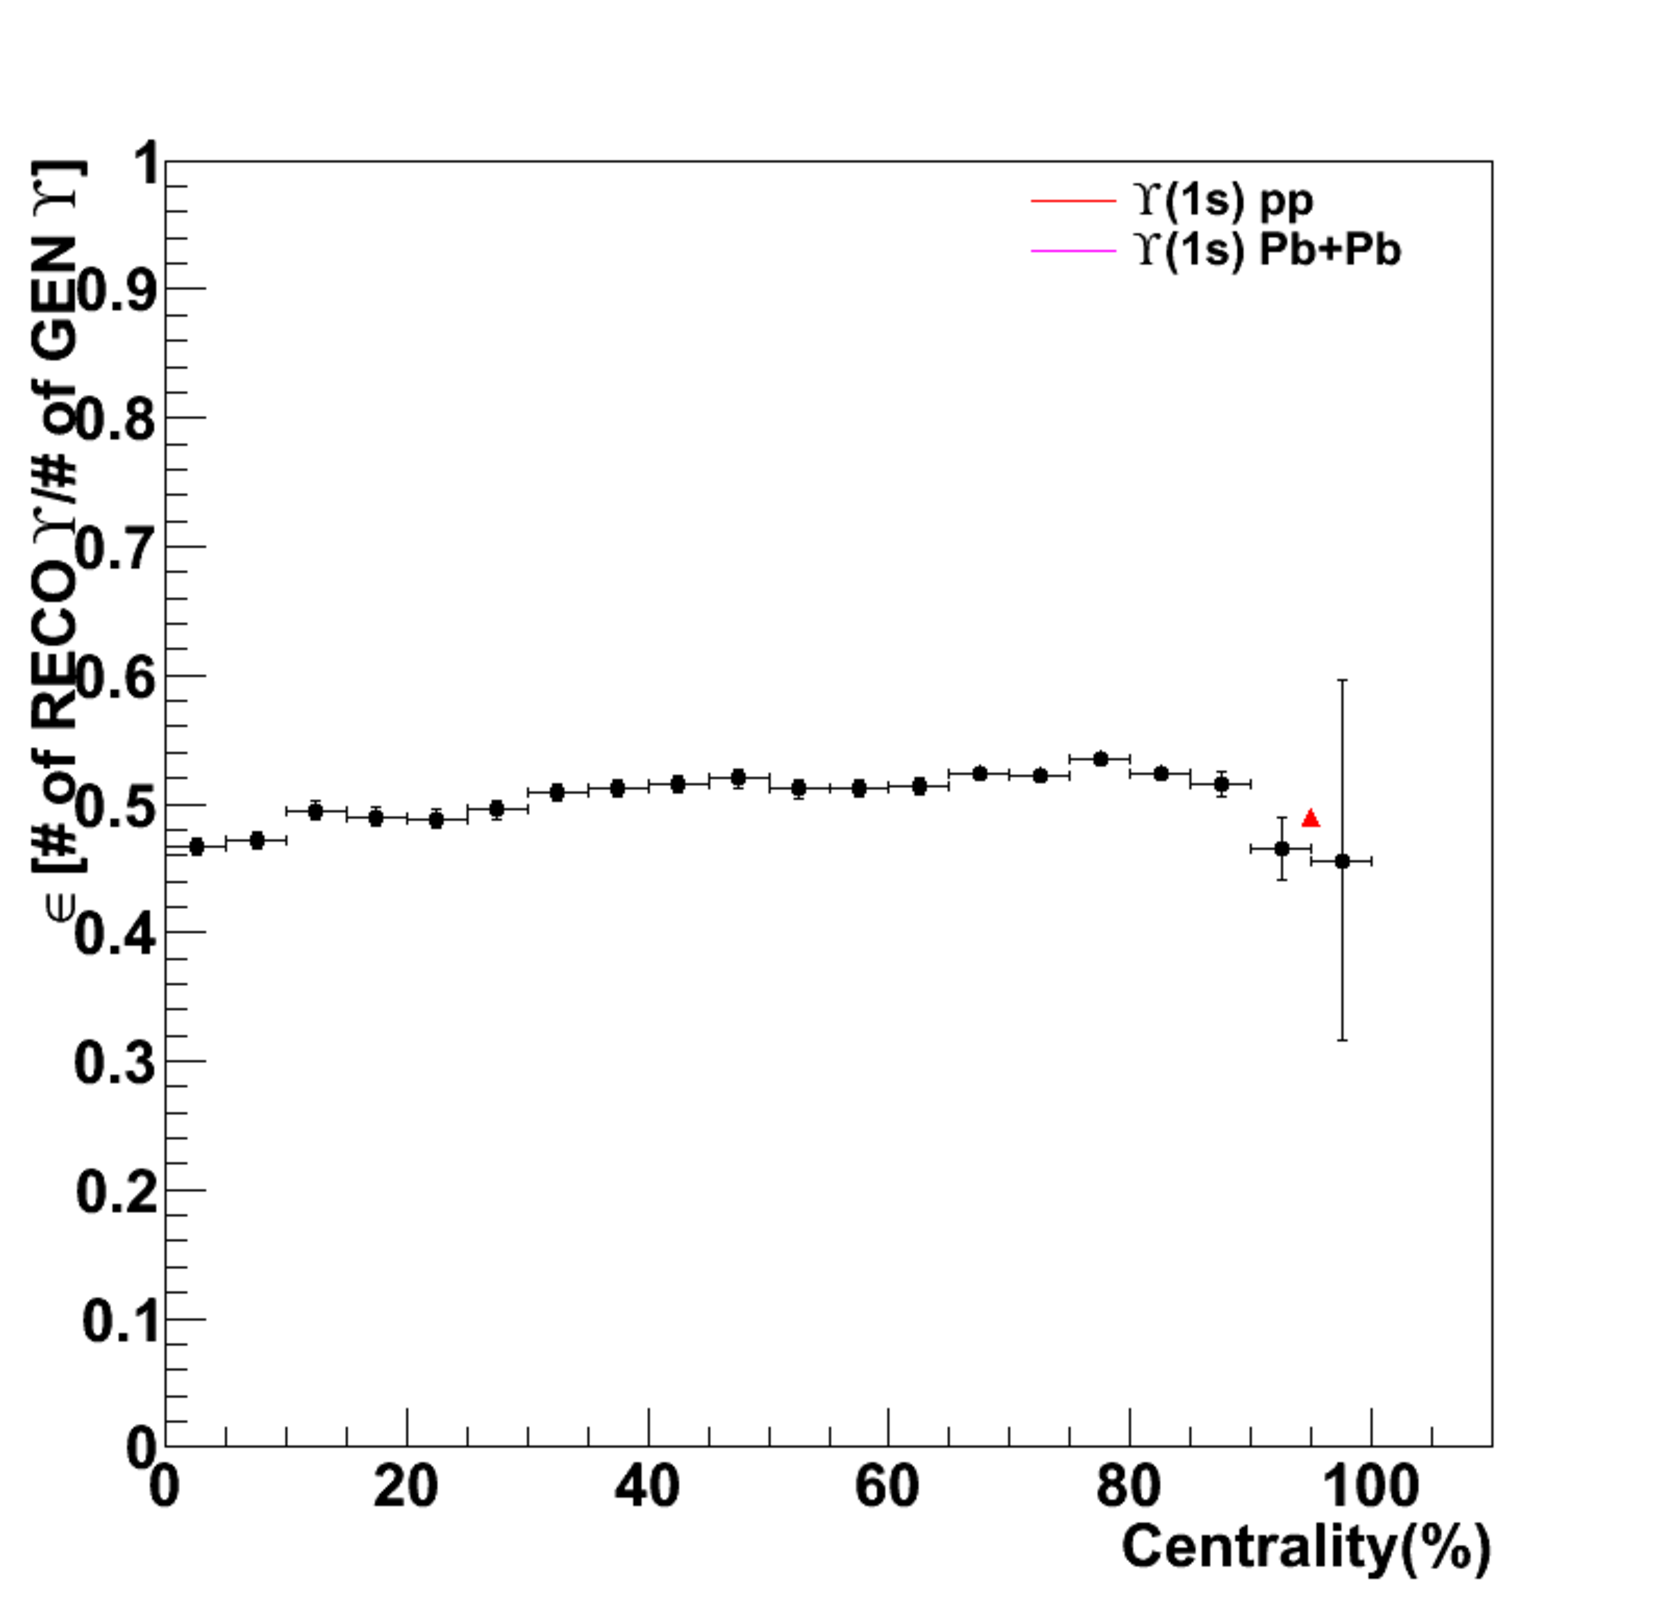
\includegraphics[angle=0,width=0.4\textwidth]{figures/efficiency/Ups1s_EffCent_pt4_finebin}\label{fig:PVtxEffCentTot}}
\hspace{5mm}
    \subfigure[Primary vertex selection efficiency. The horizontal dashed, red line indicates the \pp efficiency. (Shown for $\pt^{\Upsilon}<3\GeVc$.) ]{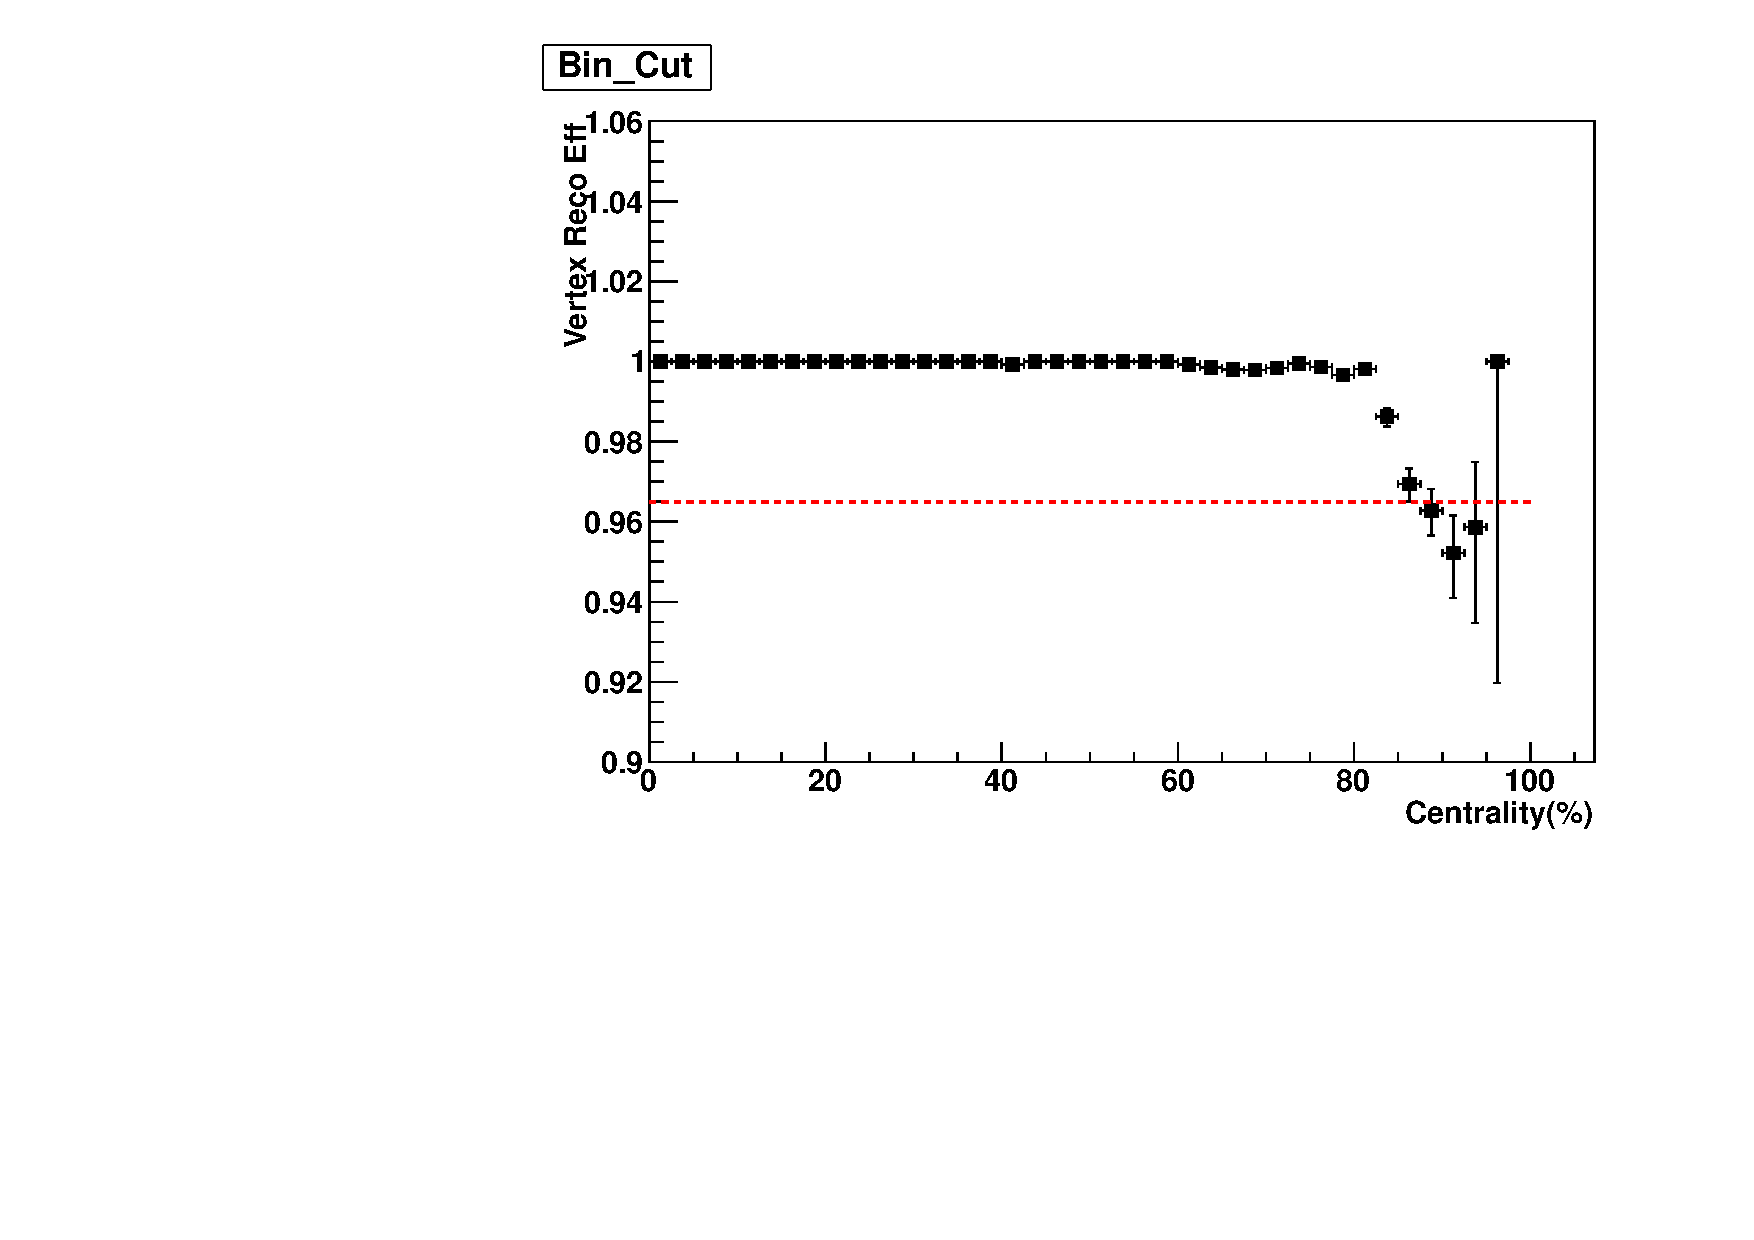
\includegraphics[angle=0,width=0.49\textwidth]{figures/efficiency/PVtxSelEff_1s_pt4}\label{fig:PVtxEffCentPVonly}}
    %\subfigure[Finer binning.]{\includegraphics[angle=0,width=0.5\textwidth]{figures/efficiency/PVtxSelEff_1s_pt4_finebin}}
    \caption{Total and primary-vertex selection efficiencies as a function of centrality, for \PbPb simulated events (shown for \PgUa,  $\pt^{\mu}>4.0\GeVc$). It illustrates an efficiency decrease for very peripheral events.}
    \label{fig:PVtxEffCent}
  \end{center}
\end{figure}

%\begin{figure}[h!]
%  \begin{center}
%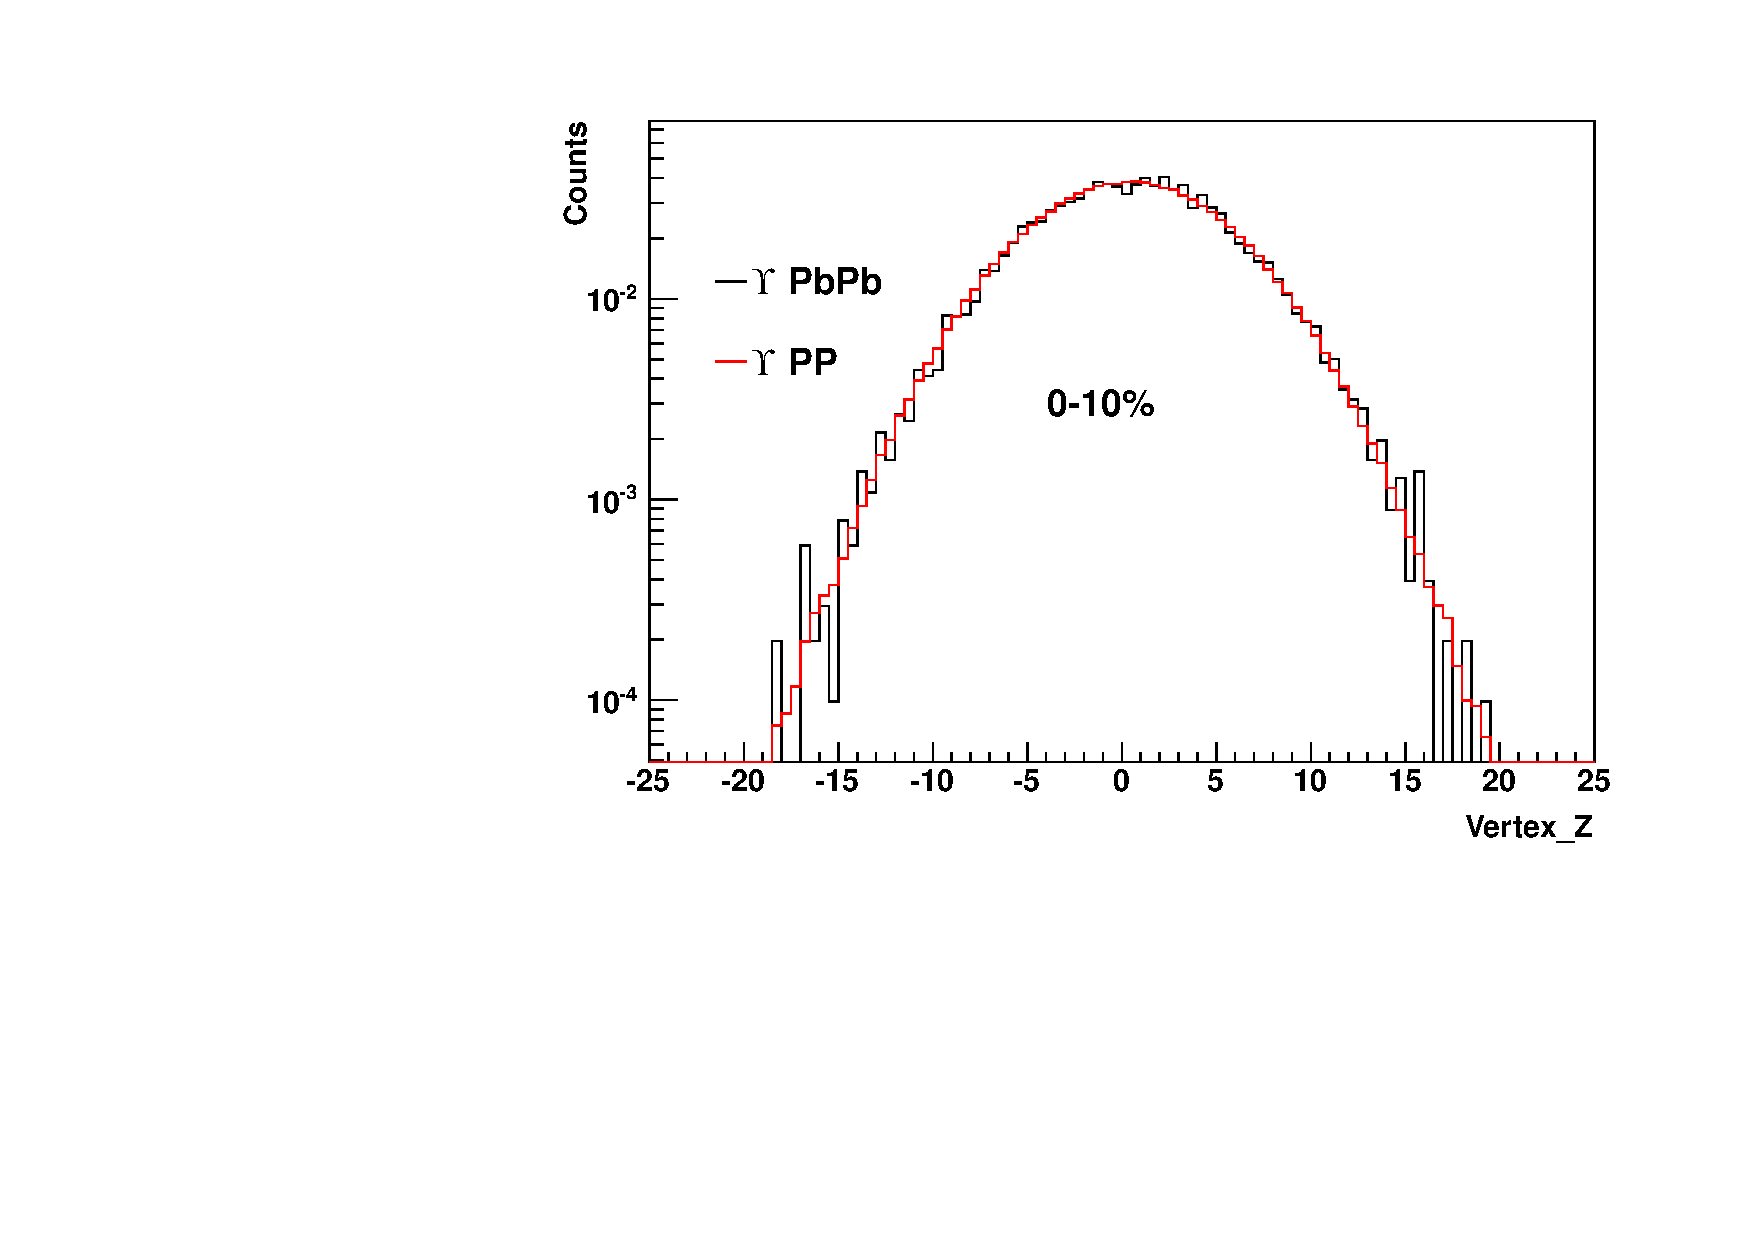
\includegraphics[angle=0,width=0.4\textwidth]{figures/efficiency/Vrtx01}
%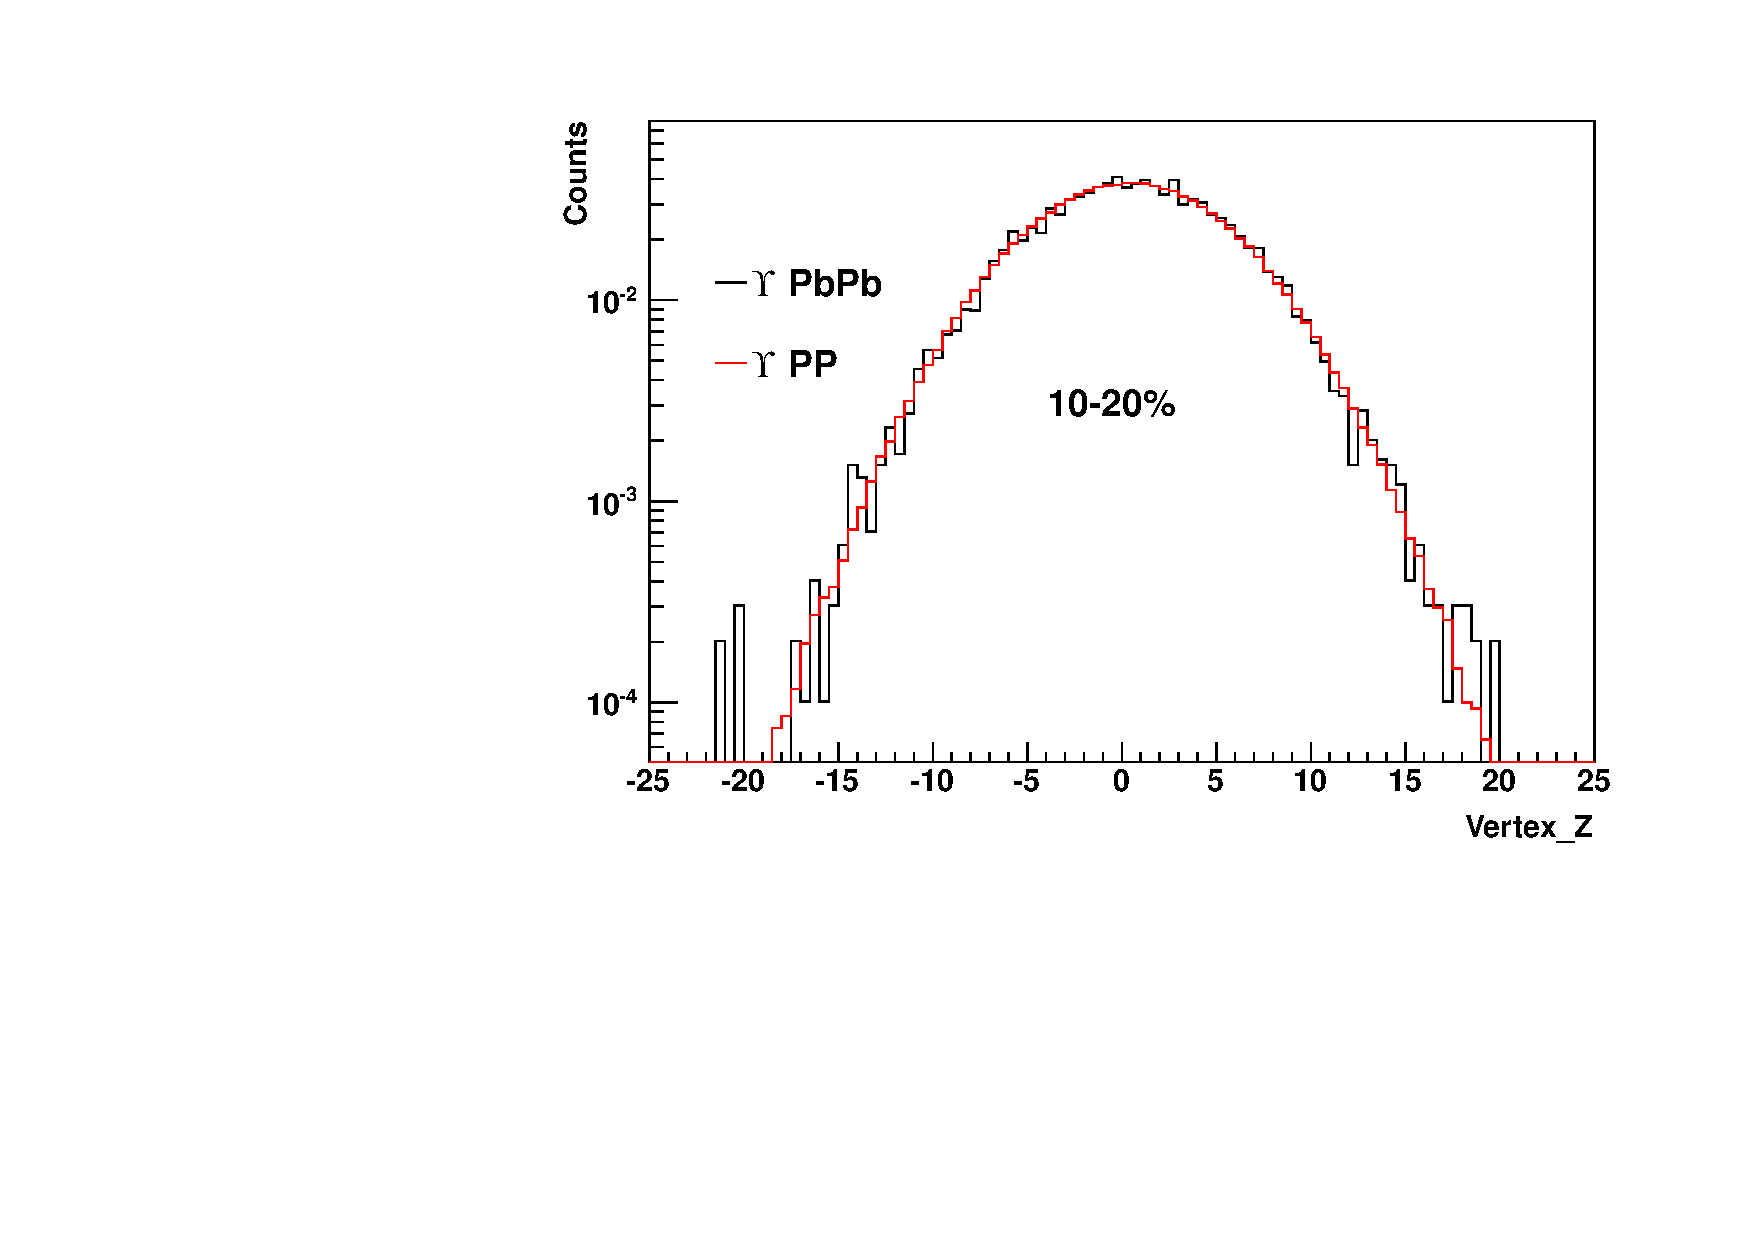
\includegraphics[angle=0,width=0.4\textwidth]{figures/efficiency/Vrtx02}
%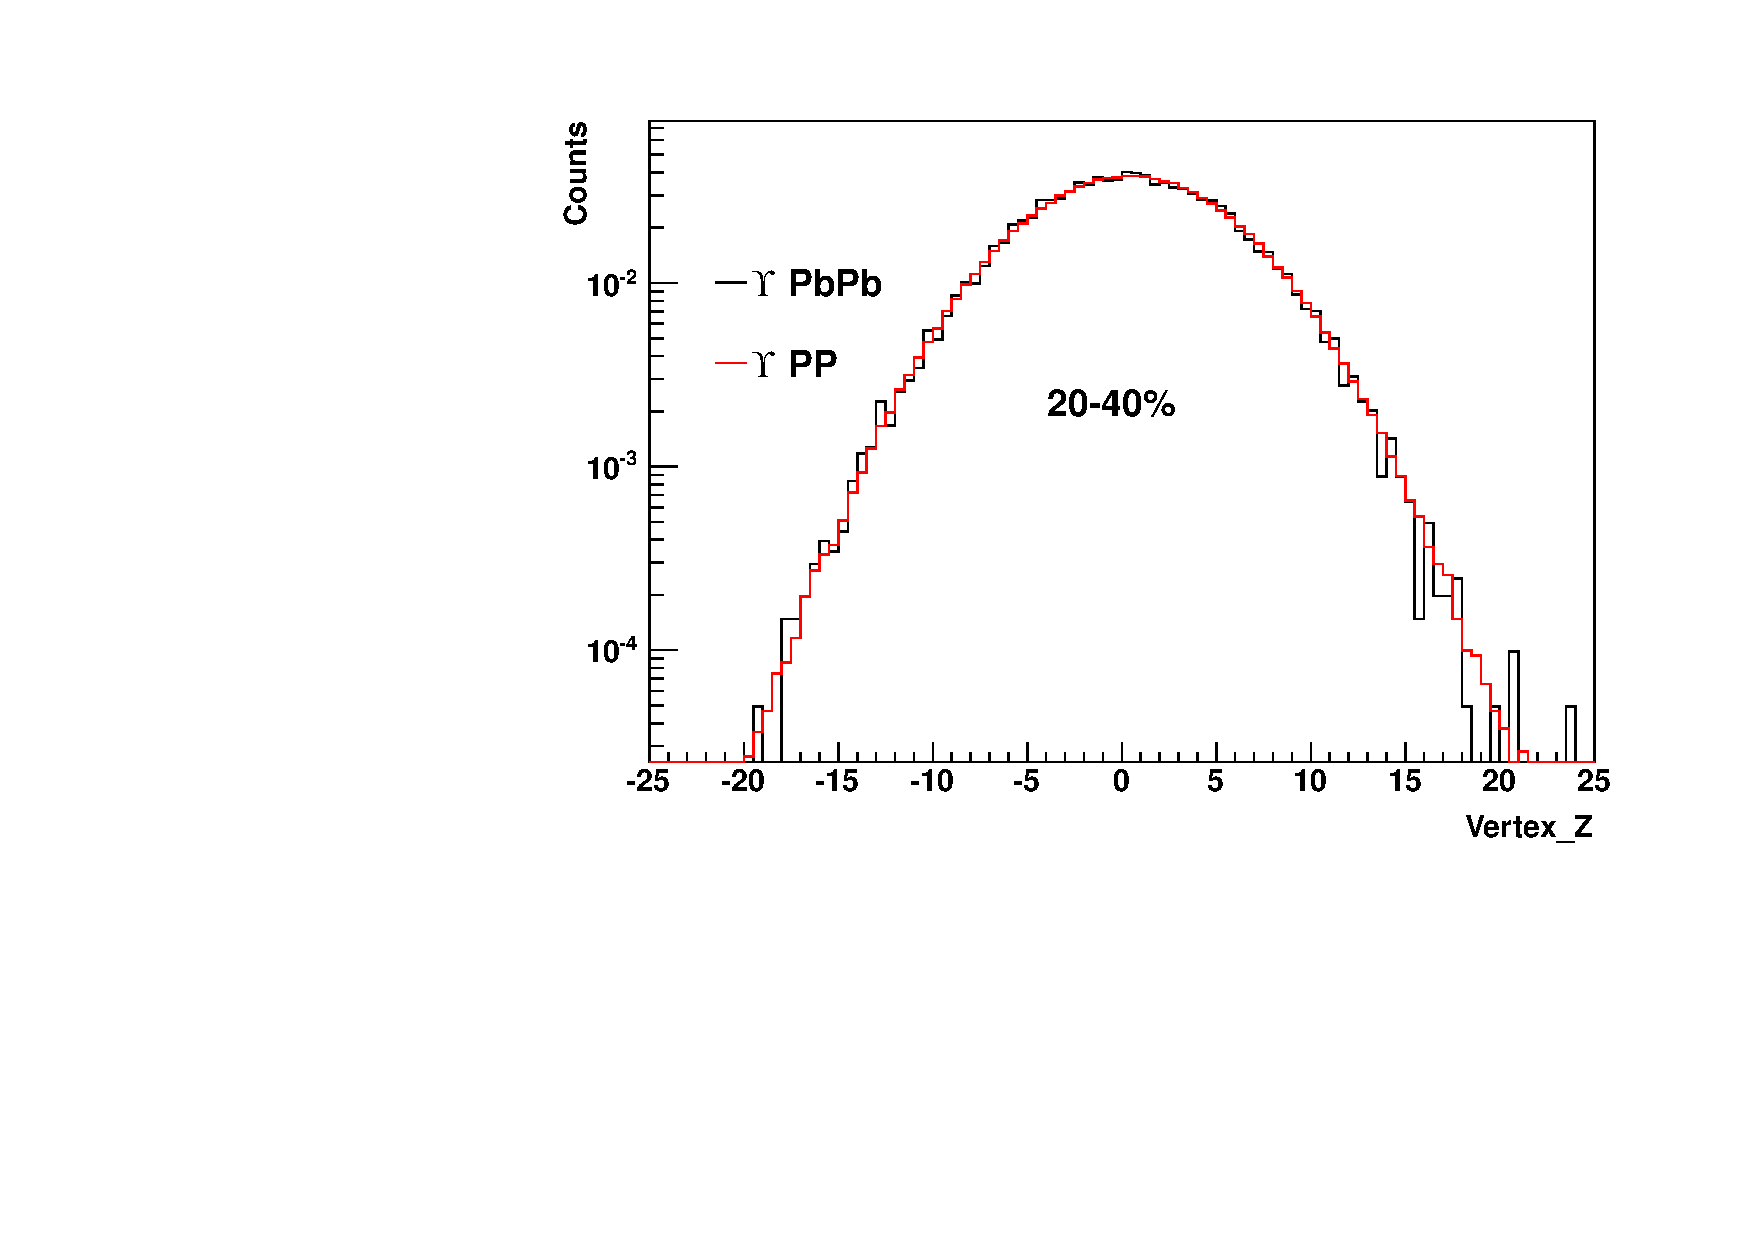
\includegraphics[angle=0,width=0.4\textwidth]{figures/efficiency/Vrtx03}
%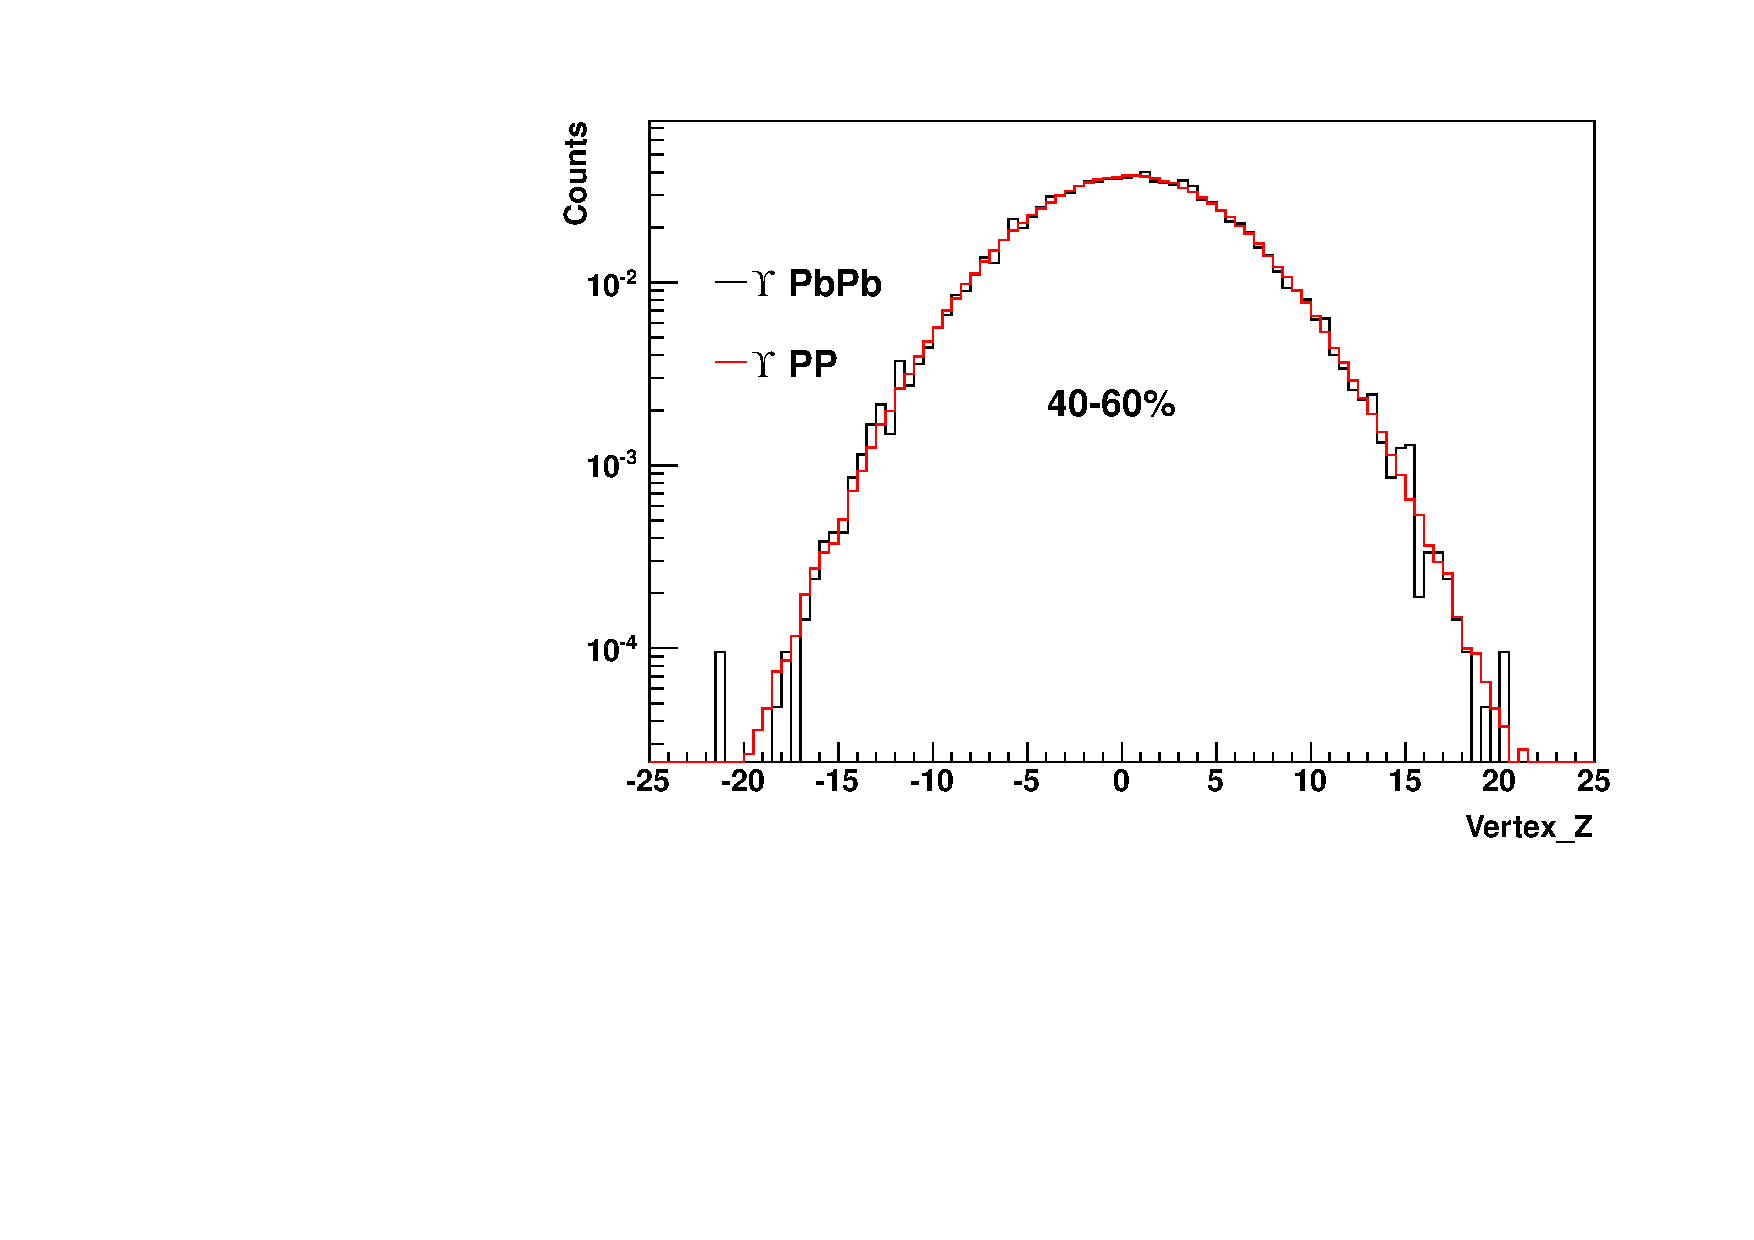
\includegraphics[angle=0,width=0.4\textwidth]{figures/efficiency/Vrtx04}
%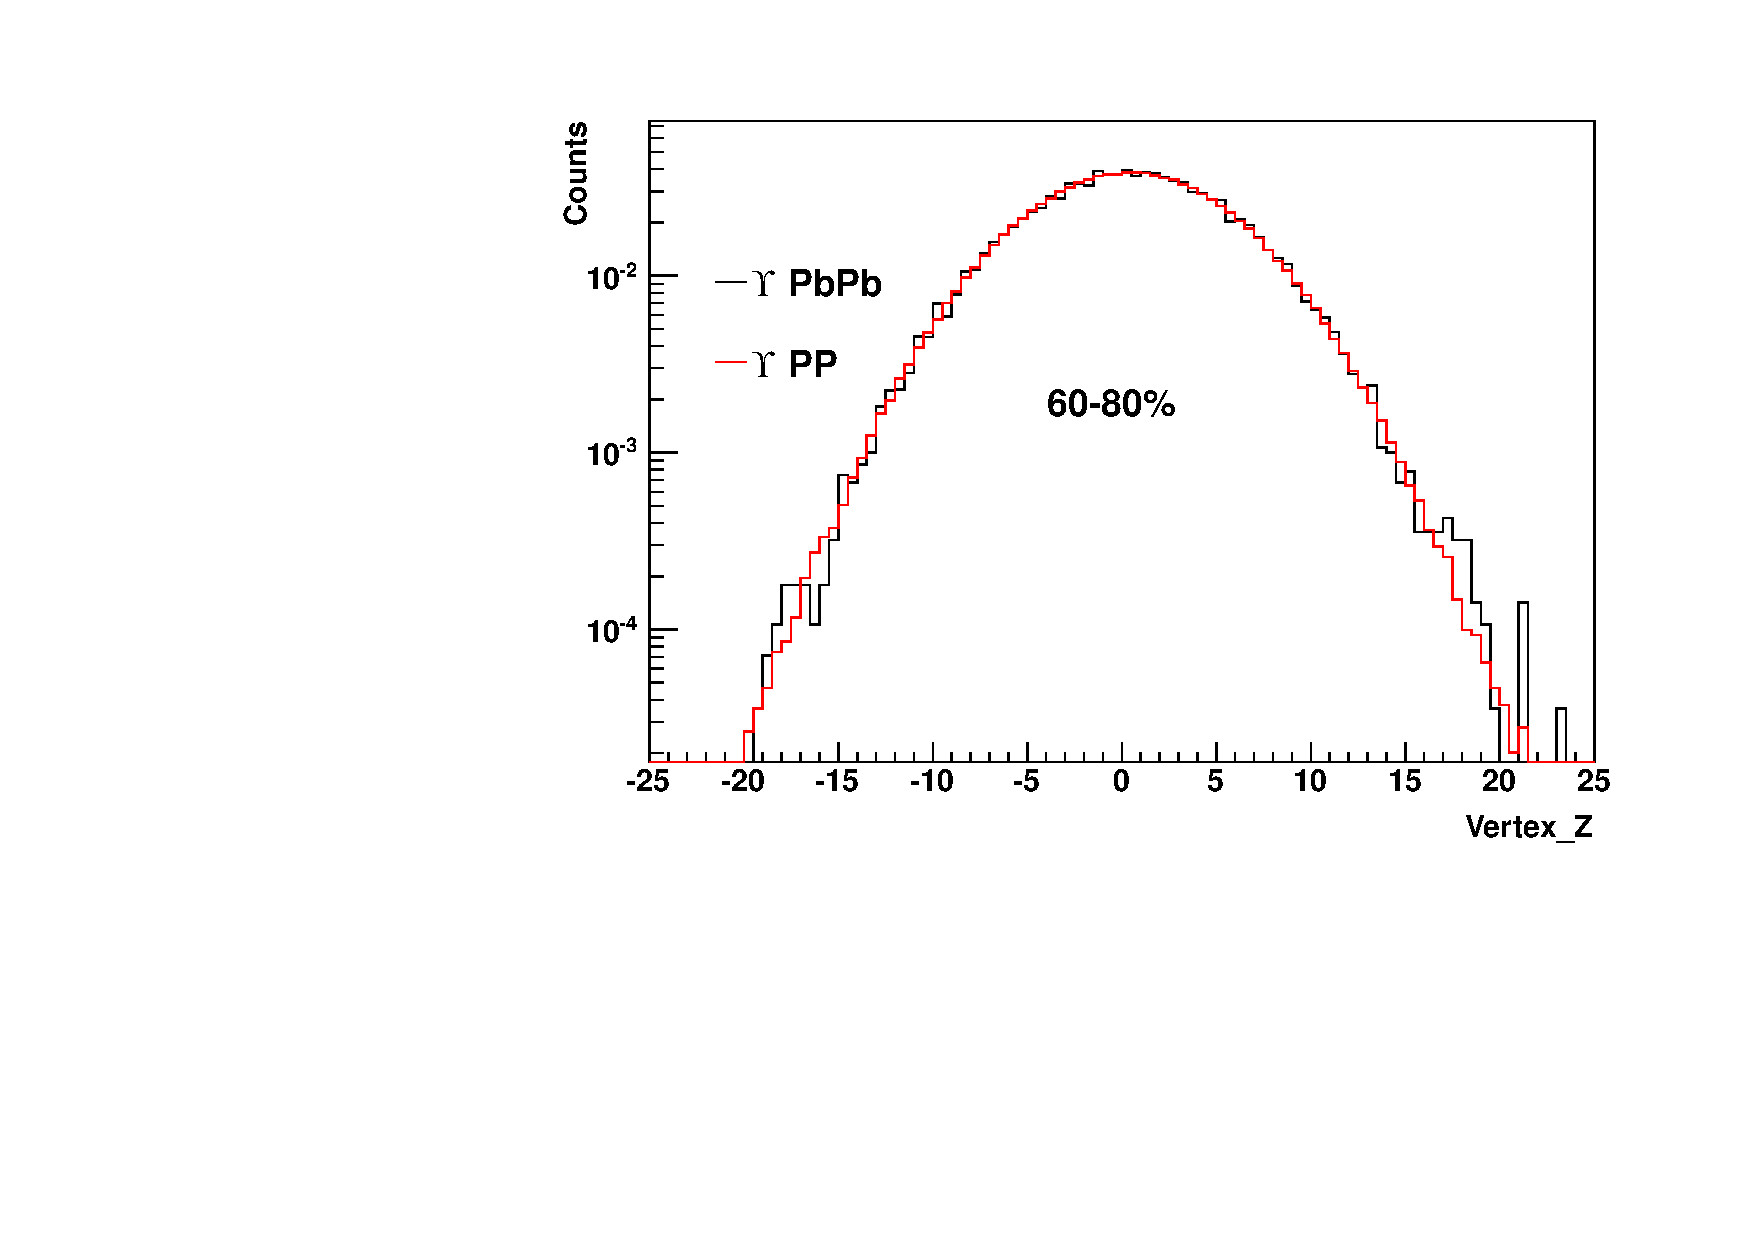
\includegraphics[angle=0,width=0.4\textwidth]{figures/efficiency/Vrtx05}
%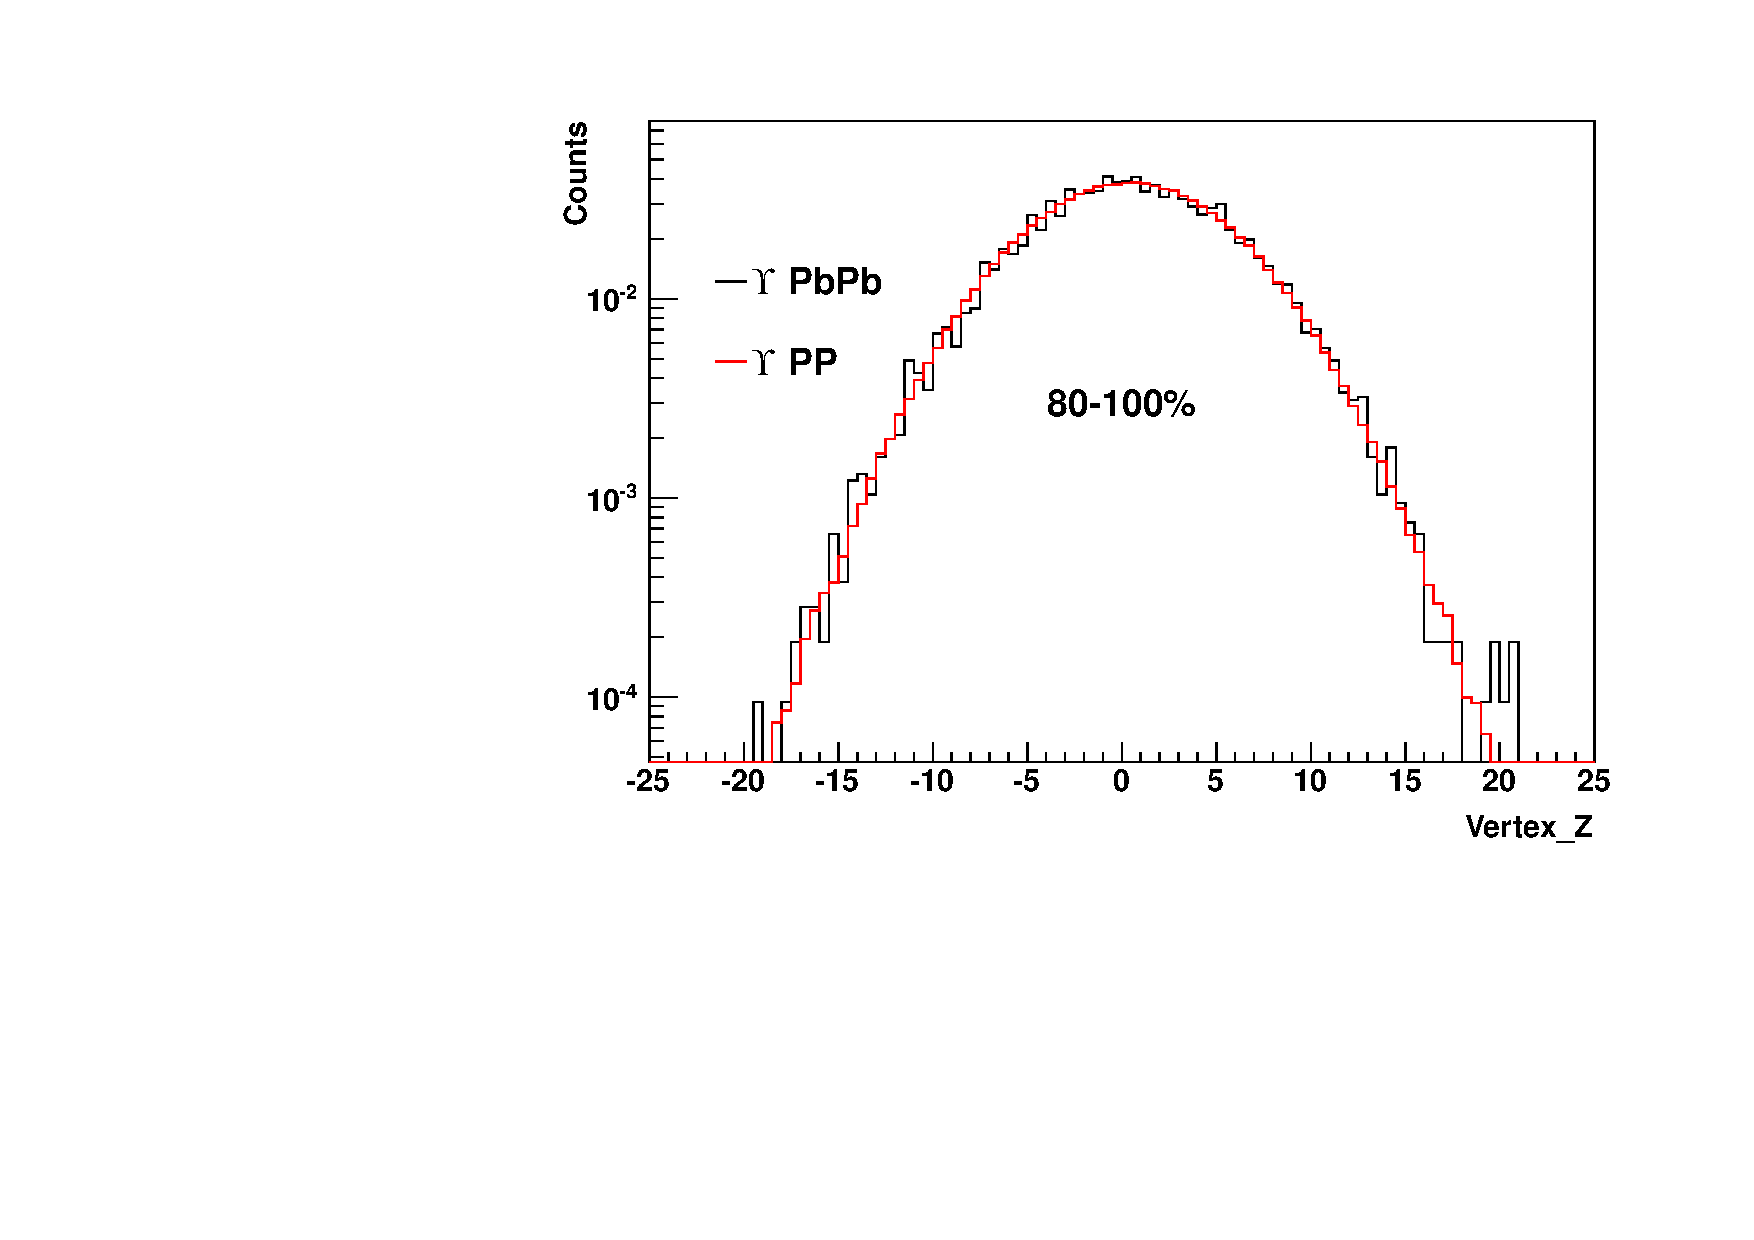
\includegraphics[angle=0,width=0.4\textwidth]{figures/efficiency/Vrtx06}
%    \caption{Primary vertex Z distribution between \PbPb and \pp MC simulation.}
 %   \label{fig:PVtxZ_Cent}
%  \end{center}
%\end{figure}


The comparison between \pp and \PbPb events, shown as the rightmost bins in \fig{fig:EffCent}, indicates a larger efficiency for \PbPb peripheral than \pp, which is not readily expected. 
This is clarified in~\fig{fig:PVtxEffCent}. 
It shows a decrease of efficiency for very peripheral ($>80\%$) events, induced by the primary vertex selection requirement.
As seen in~\fig{fig:PVtxEffCentPVonly}, the  primary vertex selection efficiency is flat in \PbPb for centralities up to about 80\% and is larger than for \pp: $99.7 \pm 0.4\%$ (\PbPb) vs $96.5 \pm 0.1\%$ (\pp).  
For peripheral \PbPb as well as for \pp collisions, which are characterized by small track multiplicities, the primary vertex selection induces inefficiencies. 
It is shown, finally in~\fig{fig:PVtxEffCentTot}, that the efficiencies for \pp and most peripheral events coincide. 
%The primary vertex Z distributions between \PbPb and \pp in MC are shown in Figure~~\fig{fig:PVtxZ_Cent}. 
%
In addition to these verifications in MC, the primary vertex selection efficiency was estimated directly in the \pp minbias dataset as well: the fraction of events found to satisfy this selection requirement is $95.9 \pm 0.8\%$, in agreement with the \pp value estimated in MC quoted above ($96.5 \pm 0.1\%$). 


\begin{figure}[h!]
  \begin{center}
   \subfigure[$\pt^\mu > 3.5\GeVc$]{\includegraphics[angle=0,width=0.5\textwidth]
%{figures/efficiency/Ups_EffRatioCent_pt35}}
{figures/efficiency/EffiRatioPt35}}
    \subfigure[$\pt^\mu > 4\GeVc$]{\includegraphics[angle=0,width=0.5\textwidth]
%{figures/efficiency/Ups_EffRatioCent_pt4}}
{figures/efficiency/EffiRatioPt40}}
    \caption{Ratios of total efficiencies as a function of centrality, comparing \PbPb and \pp.}
    \label{fig:EffRatioCent_pt}
  \end{center}
\end{figure}


Figure~\ref{fig:EffRatioCent_pt} shows the centrality dependence of the ${\PgUa}/{\PgUb}$ ratio of total efficiencies  in \PbPb, compared with the same in \pp.
%
In order to estimate possible efficiency corrections to the double ratio %$\chi_2$ 
observable,  we calculate the double ratio of efficiencies: 

\[
\chi \; 
\text{efficiency correction} \equiv \frac{ \varepsilon_{\PgUa} / \varepsilon_{\PgUb} \mid_\PbPb} { \varepsilon_{\PgUa} / \varepsilon_{\PgUb} \mid_\pp} \,.
\]

The value of such a possible correction, evaluated for different centrality bins, is shown in 
Table~\ref{Tab:DRatioShapePtRap}. %Table~\ref{Tab:DR_CF}. 
It is found to lie in the range (0.98 to 1.03). This is found to be consistent and fluctuating about unit; the variations are small and negligible compared to the statistical uncertainty expected for the double ratio measurement. 

%THIS TABLE should be replaced by
%\begin{table}[h!]
%\begin{center}
%\caption{Efficiency correction factor for the double ratio, $\chi_2$.}
%\label{Tab:DR_CF}
%\begin{tabular}{c|c|c}
%  \hline
%   centrality              & correction factor & relative Syst.  \\
%  \hline
%   $[0-100\%]$            &$1.000\pm0.002$    &$0.003\%$ \\
%
%   $[0-5\%]$              &$0.999 \pm 0.002$   &$0.0639\%$ \\
%   $[5-10\%]$             &$0.995 \pm 0.0002$     &$0.467\%$ \\
%   $[10-20\%]$            &$1.022 \pm 0.002$   &$1.82\%$ \\
%   $[20-30\%]$            &$0.992 \pm 0.002$   &$0.792\%$\\
%   $[30-40\%]$            &$1.010 \pm 0.00005$      &$1.22\%$\\
%   $[40-50\%]$            &$1.020 \pm 0.002$    &$1.8\%$\\
%   $[50-100\%]$           &$0.988 \pm 0.002$   &$1.26\%$\\
%\hline
%\end{tabular}
%\end{center}
%\end{table}
%TBD: add stat and syst error to this calculation

Though we embed \PgU in all centralities in a democratic way, the final MC centrality distribution, shown in  \fig{fig:Centrality}, is not flat. 
%The number of generated $\PgU$ particles versus centrality, in MC simulation, is not flat as can be seen in .  
This is due to the fact that the variable used to define the centrality bins for an event, the number of hits in the Forward Hadronic Calorimeters (HF), is based upon the simulated minimum bias HYDJET \PbPb collision. Since a \pp collision is embedded into that minimum bias event, the underlying event leaves extra hits in the HF, which shifts the number of HF hits up, leaving less most peripheral events. This shift can be most strongly seen for the $>70\%$ bins. 
%bins from 30-40.  
%In the study with respect to centrality, since the events with centralities between 50-100\% (bins 20-40) are binned together, this shift stays within the peripheral bin.

\begin{figure}[h]
  \begin{center}
  %    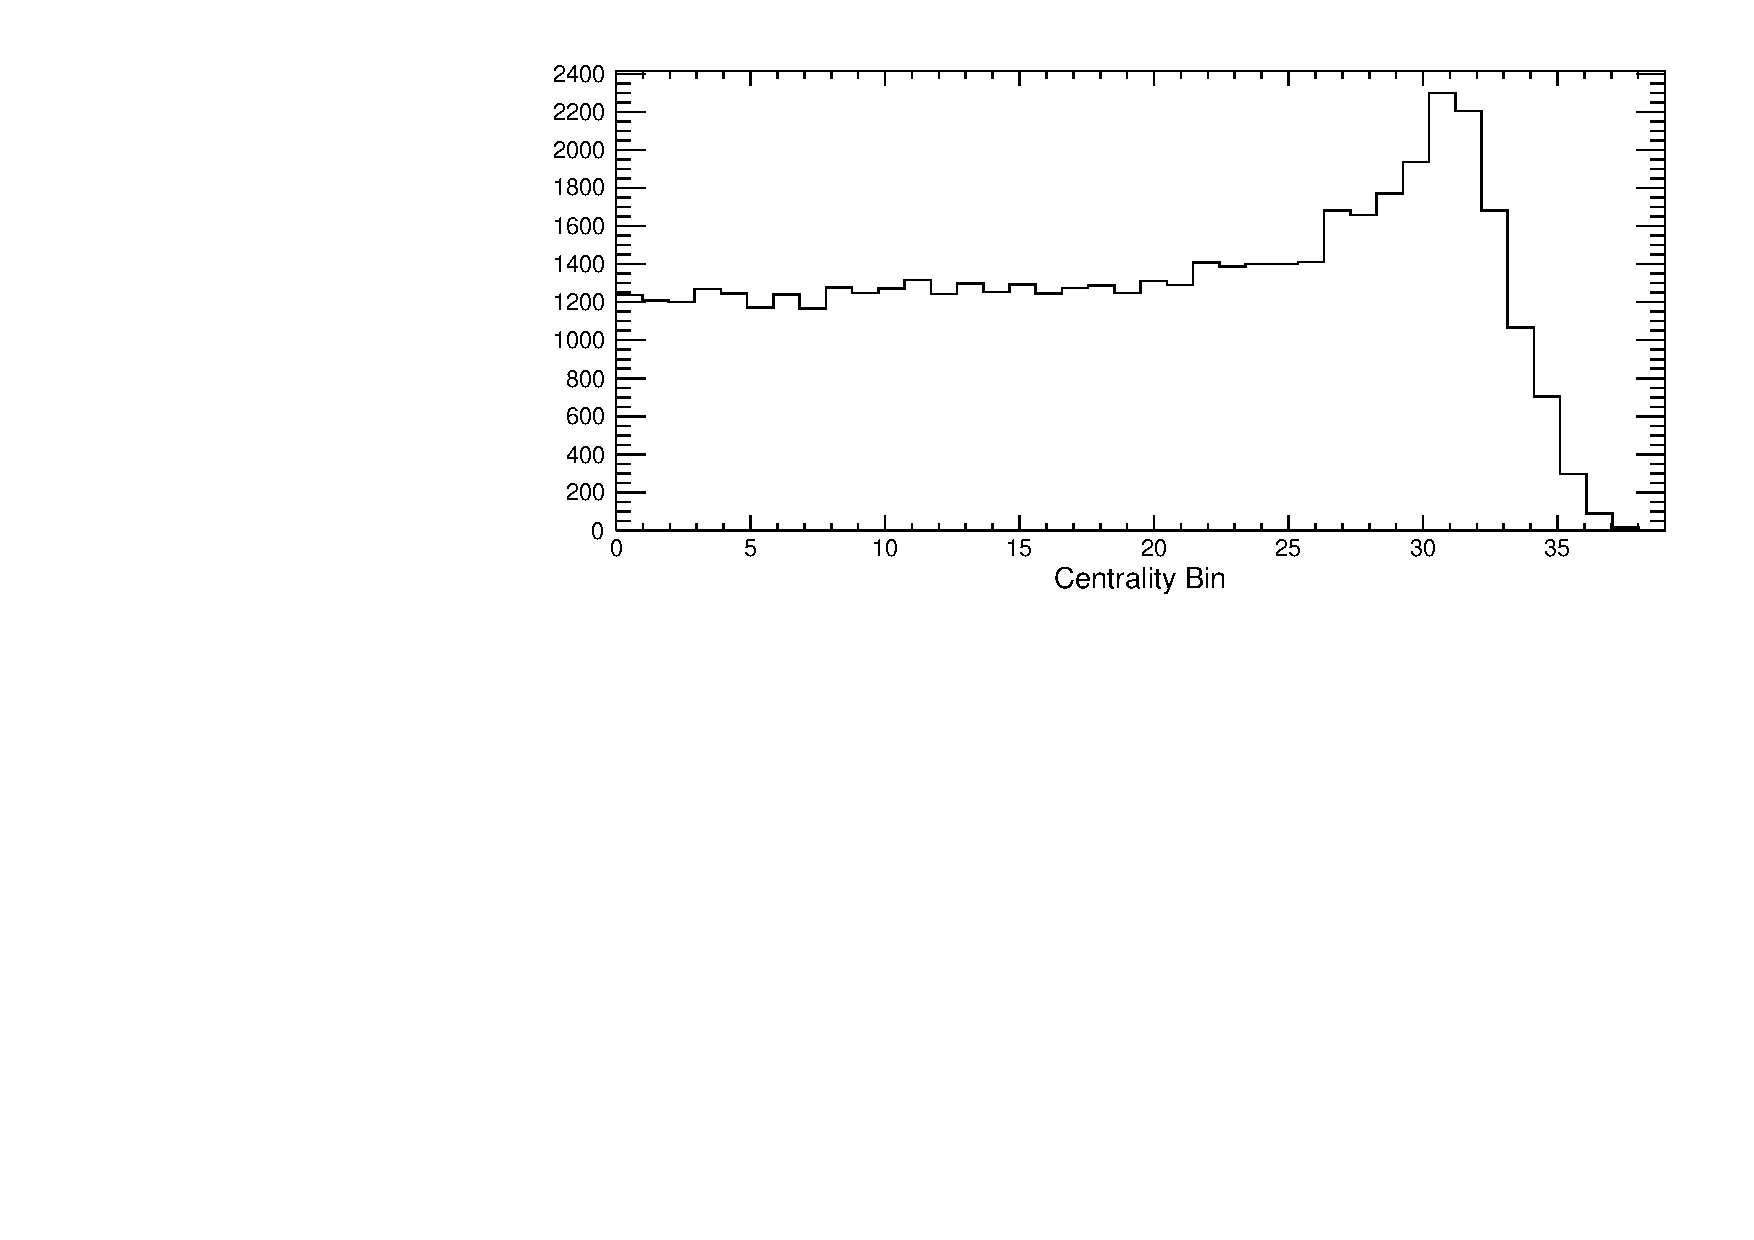
\includegraphics[angle=0,width=0.8\textwidth]{figures/efficiency/Centrality_PbPb}\hspace{1em}
    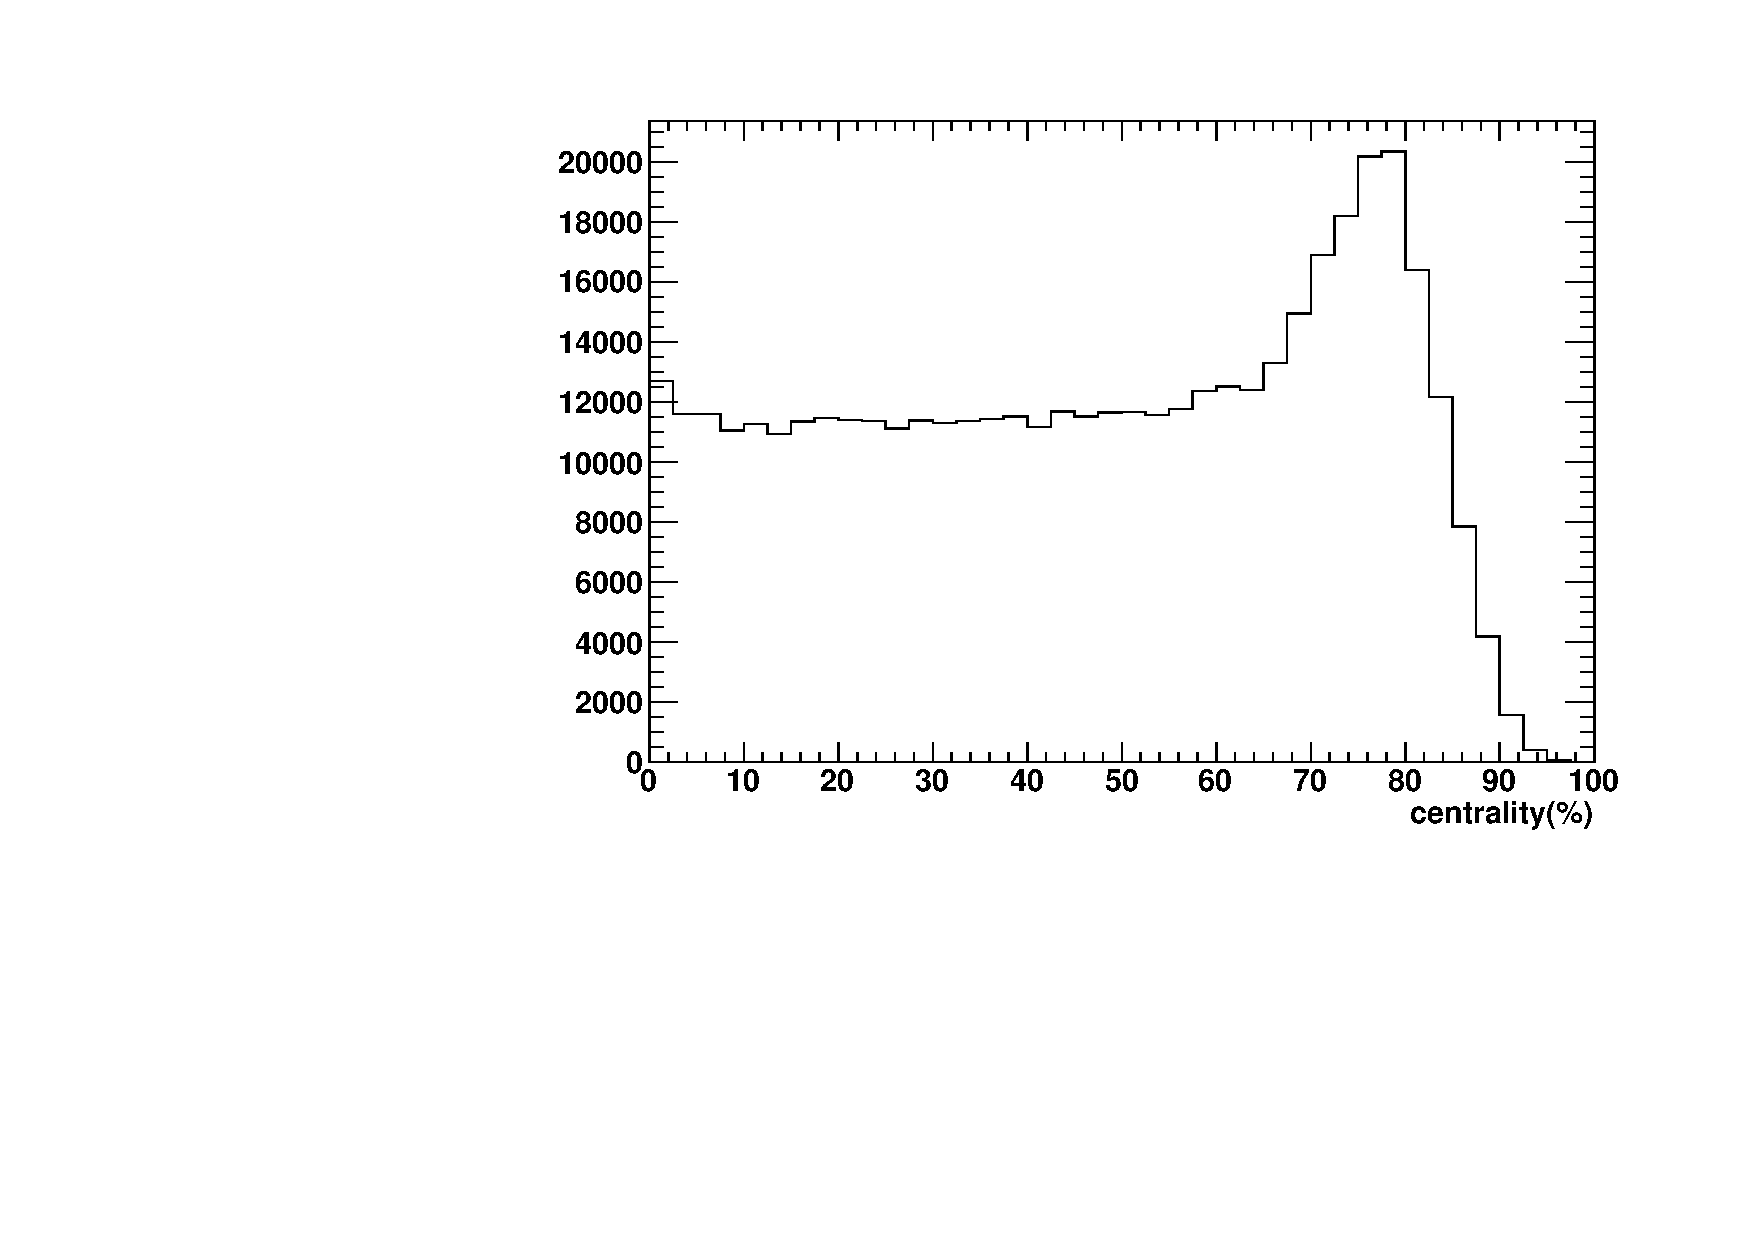
\includegraphics[angle=0,width=0.8\textwidth]{figures/efficiency/CentraltyPerc}\hspace{1em} 
    \caption{Shape of the event centrality distribution in simulation. 
    %Each centrality bin corresponds to 2.5\% of the centrality spectrum.  The zero centrality bin corresponds to 0\% or the most central collisions, and the 40 centrality bin corresponds to 100\% or the most peripheral collisions. The non-flatness of the shape in MC is explained in the text.}
 The non-flatness of the shape in MC is explained in the text.}
    \label{fig:Centrality}
  \end{center}
\end{figure}


%TBD: the description of MC should go in the correspondiing chapter
%\subsection{Datasets}
%\label{subsec:datasets}

%The datasets used are Monte Carlo generated samples, where each event is produced by taking a simulated \pp collision resulting in an \PgU decaying into two muons, and embedding into HYDJET minimum bias data at 2.76 TeV (in order to match the \PgU production from the Heavy Ion data run). All of the $\PgU s$ in the datasets have realistic $p_{T}$ and $y$ distributions and the PbPb datasets are thrown flat with centrality. The \pt range for these Ys is $0 < \pt < 3$ in all cases.

Figures~\ref{fig:muon_properties_4_0} and~\ref{fig:muon_properties_3_5} show the kinematic distributions of the dimuons and single muons from $\PgUa$ and $\PgUb$ decays, selected with the muon kinematic cut $\pt > 4.0\GeVc$ and $\pt > 3.5\GeVc$ respectively.
The most noticeable difference is the softer \pt distribution for $\PgUa$, which arises as expected from the higher $\PgUb$ mass. 

\begin{figure}[h]
  \begin{center}
    \subfigure[\PbPb MC simulation, with 68,100 \PgUa and 50,000 \PgUb.]{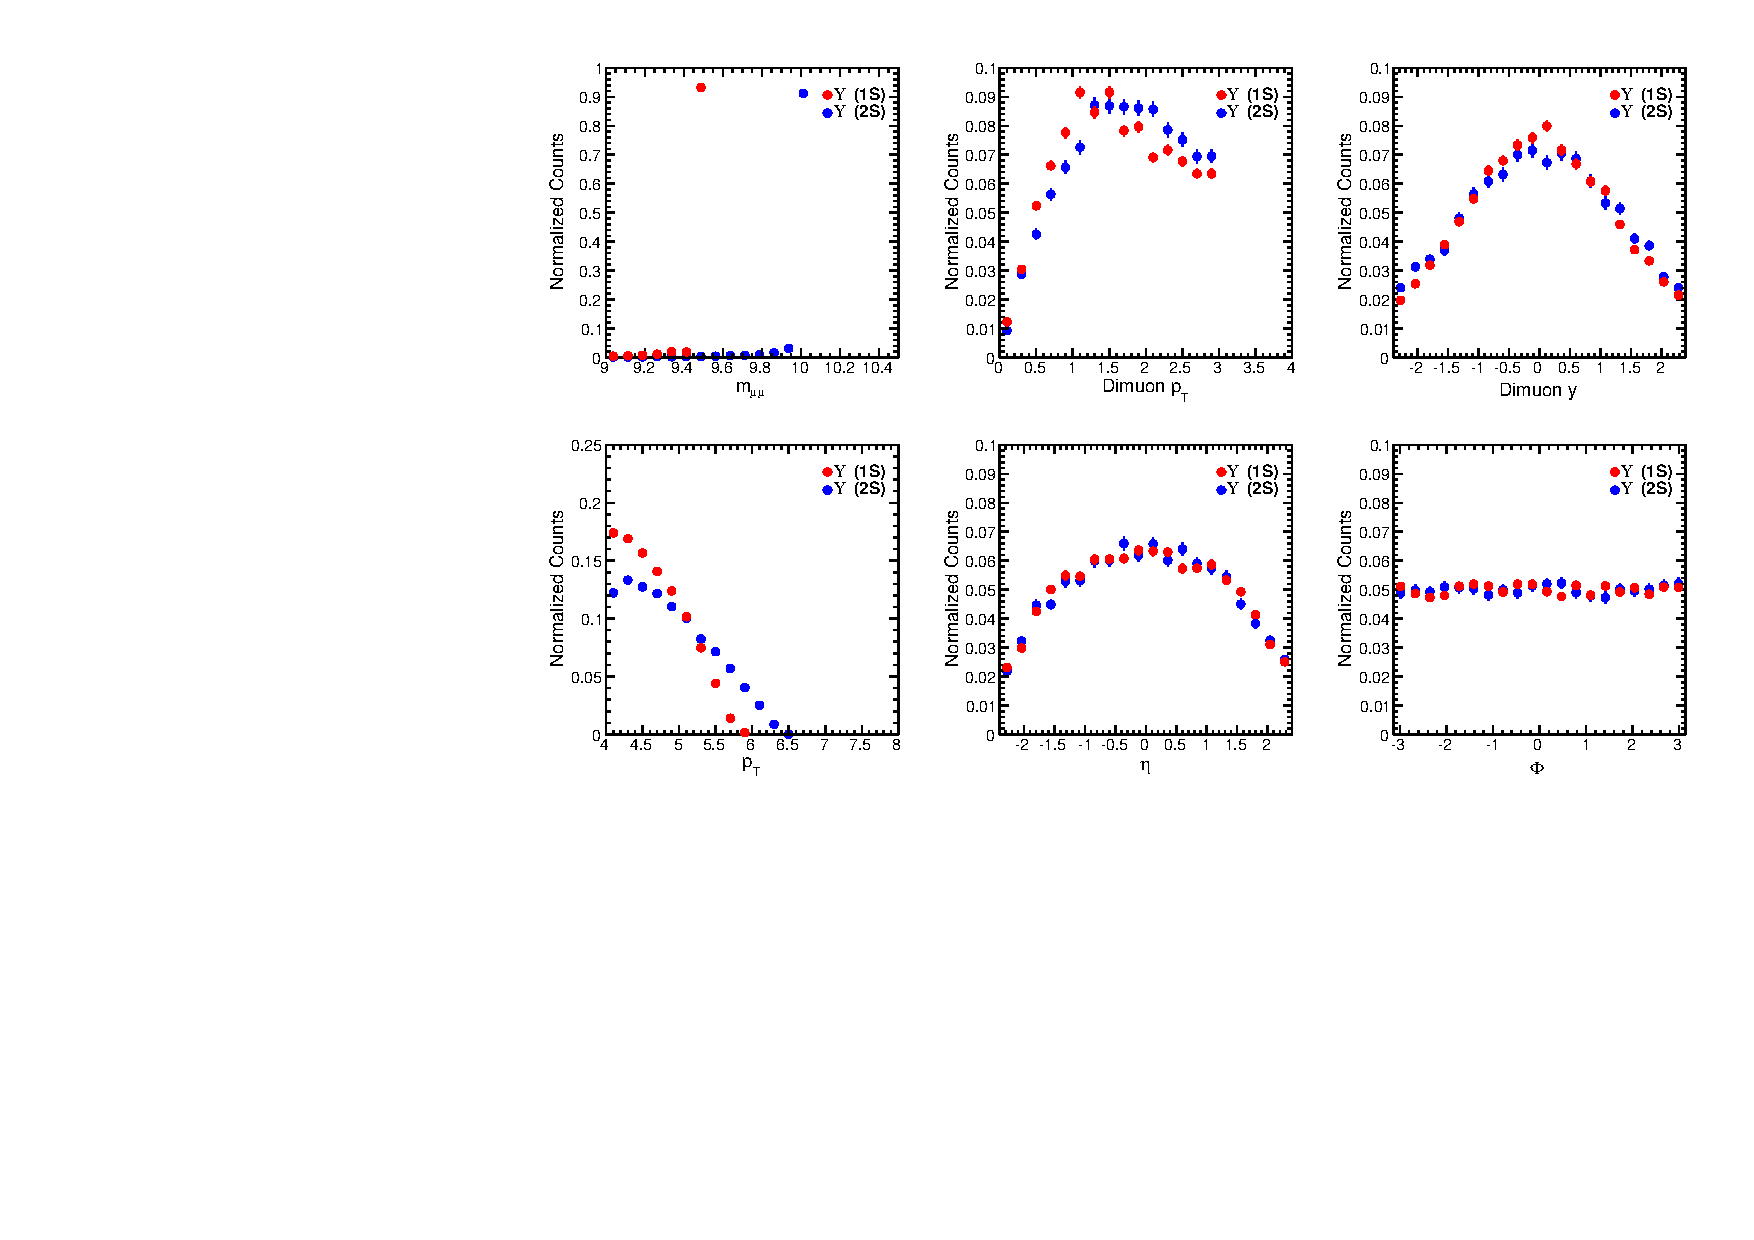
\includegraphics[angle=0,width=1.0\textwidth]{figures/efficiency/Plots_for_Upsilon_PbPb_4}\label{fig:muon_properties_PbPb_4_0}}\\
%    \caption{(top row) Normalized mass, $p_{T}$ and y distributions of the generated \PgUa and \PgUb in \PbPb events. (bottom row) Normalized $p_{T}$, $\eta$ and $\phi$ distributions for the individual muons.
%The muon kinematic requirement $\pt > 4.0\GeVc$ is applied. 
%}
%    
%  \end{center}
%\end{figure}
%
%\begin{figure}[h]
%  \begin{center}
    \subfigure[\pp MC simulation, with 3,200 \PgUa and 5,500 \PgUb.]{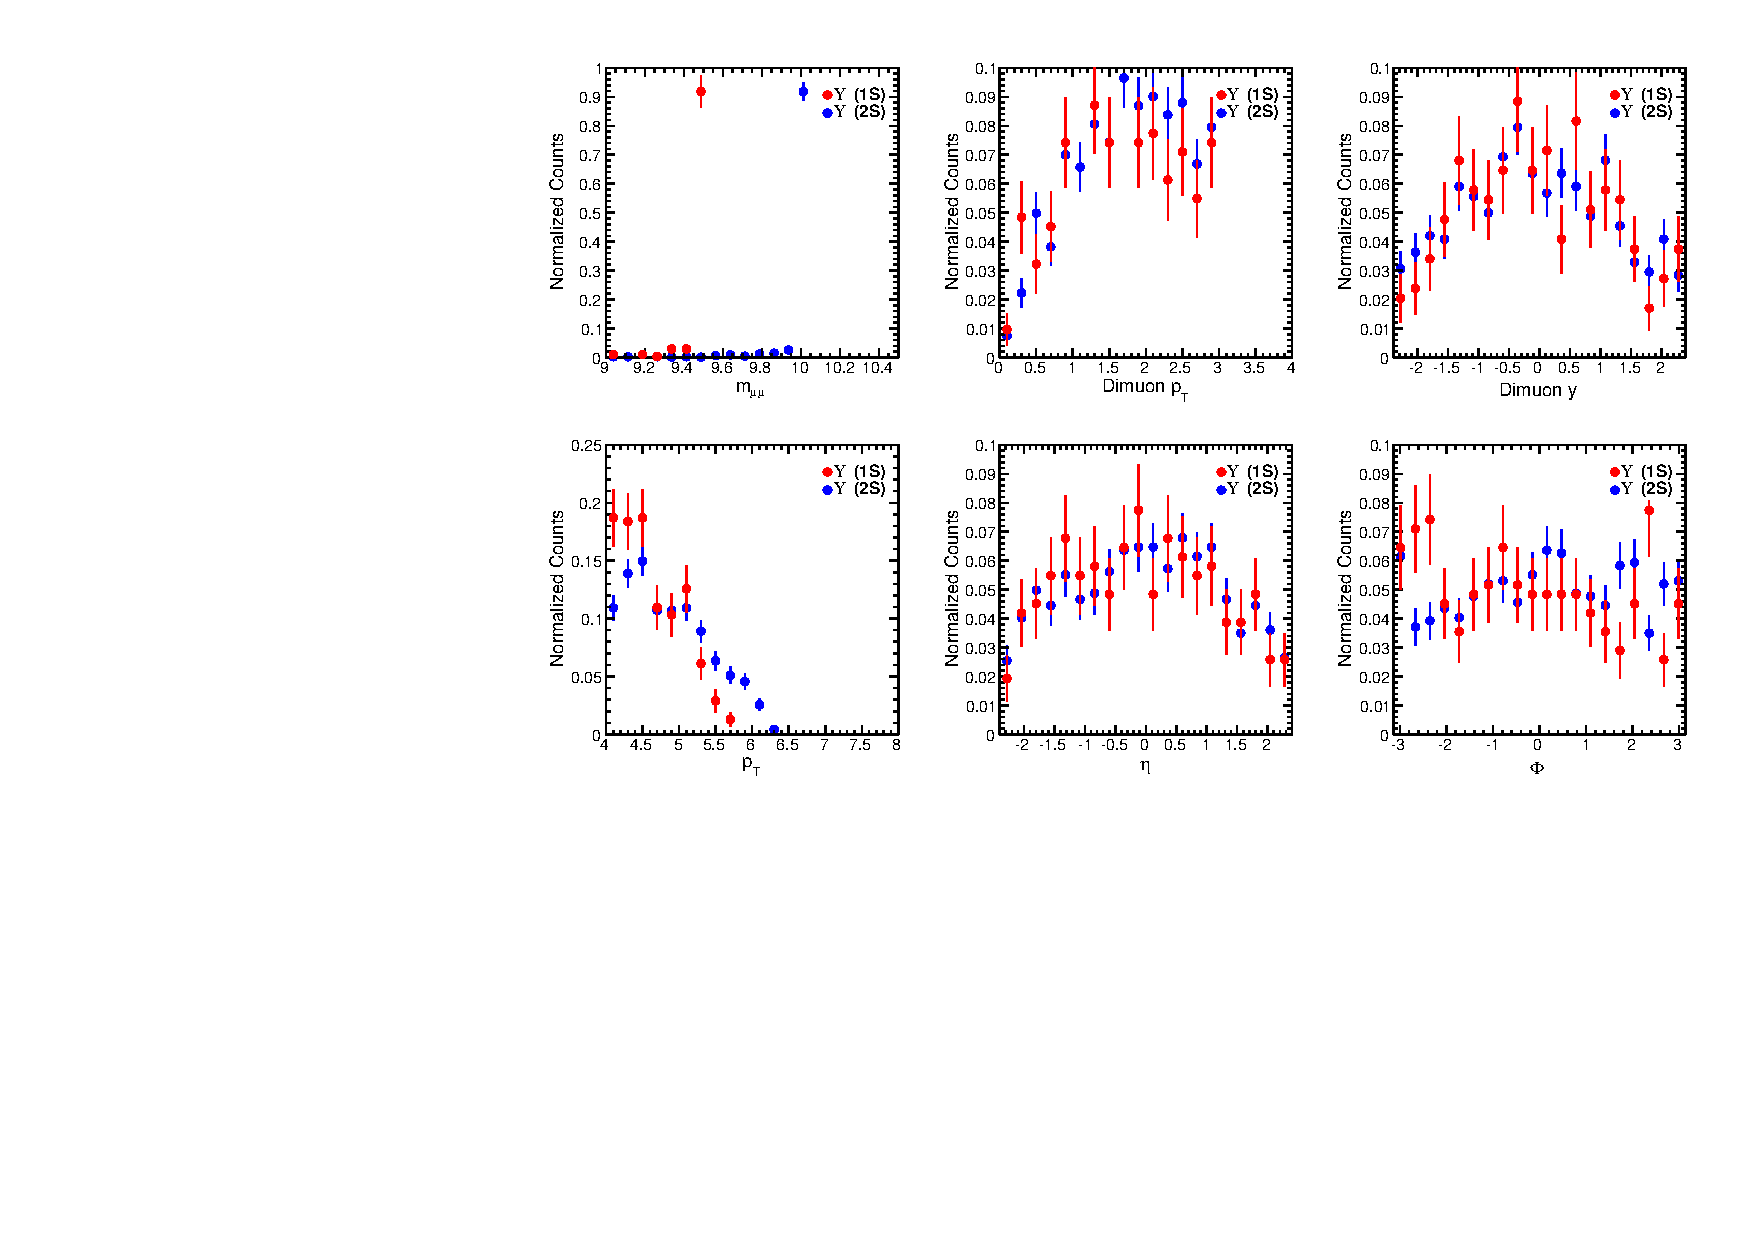
\includegraphics[angle=0,width=1.0\textwidth]{figures/efficiency/Plots_for_Upsilon_pp_4}\label{fig:muon_properties_pp_4_0}}
    %\caption{(top row) Normalized mass, $p_{T}$ and y distributions of the generated \PgUa and \PgUb in \pp events. (bottom row) Normalized $p_{T}$, $\eta$ and $\phi$ distributions for the individual muons.
%The muon kinematic requirement $\pt > 4.0\GeVc$ is applied. 
%}
    \caption{Comparison of \PgUa and \PgUb kinematic distributions in \PbPb and \pp MC simulation: 
invariant mass, \pt and $y$ di-muon normalized distributions, and 
$\pt$, $\eta$ and $\phi$ single-muon normalized distributions.
%is different than the MC due to the background being included.
The muon kinematic requirement $\pt > 4.0\GeVc$ is applied. 
}
    \label{fig:muon_properties_4_0}
  \end{center}
\end{figure}

\begin{figure}[h]
  \begin{center}
    \subfigure[\PbPb MC simulation]{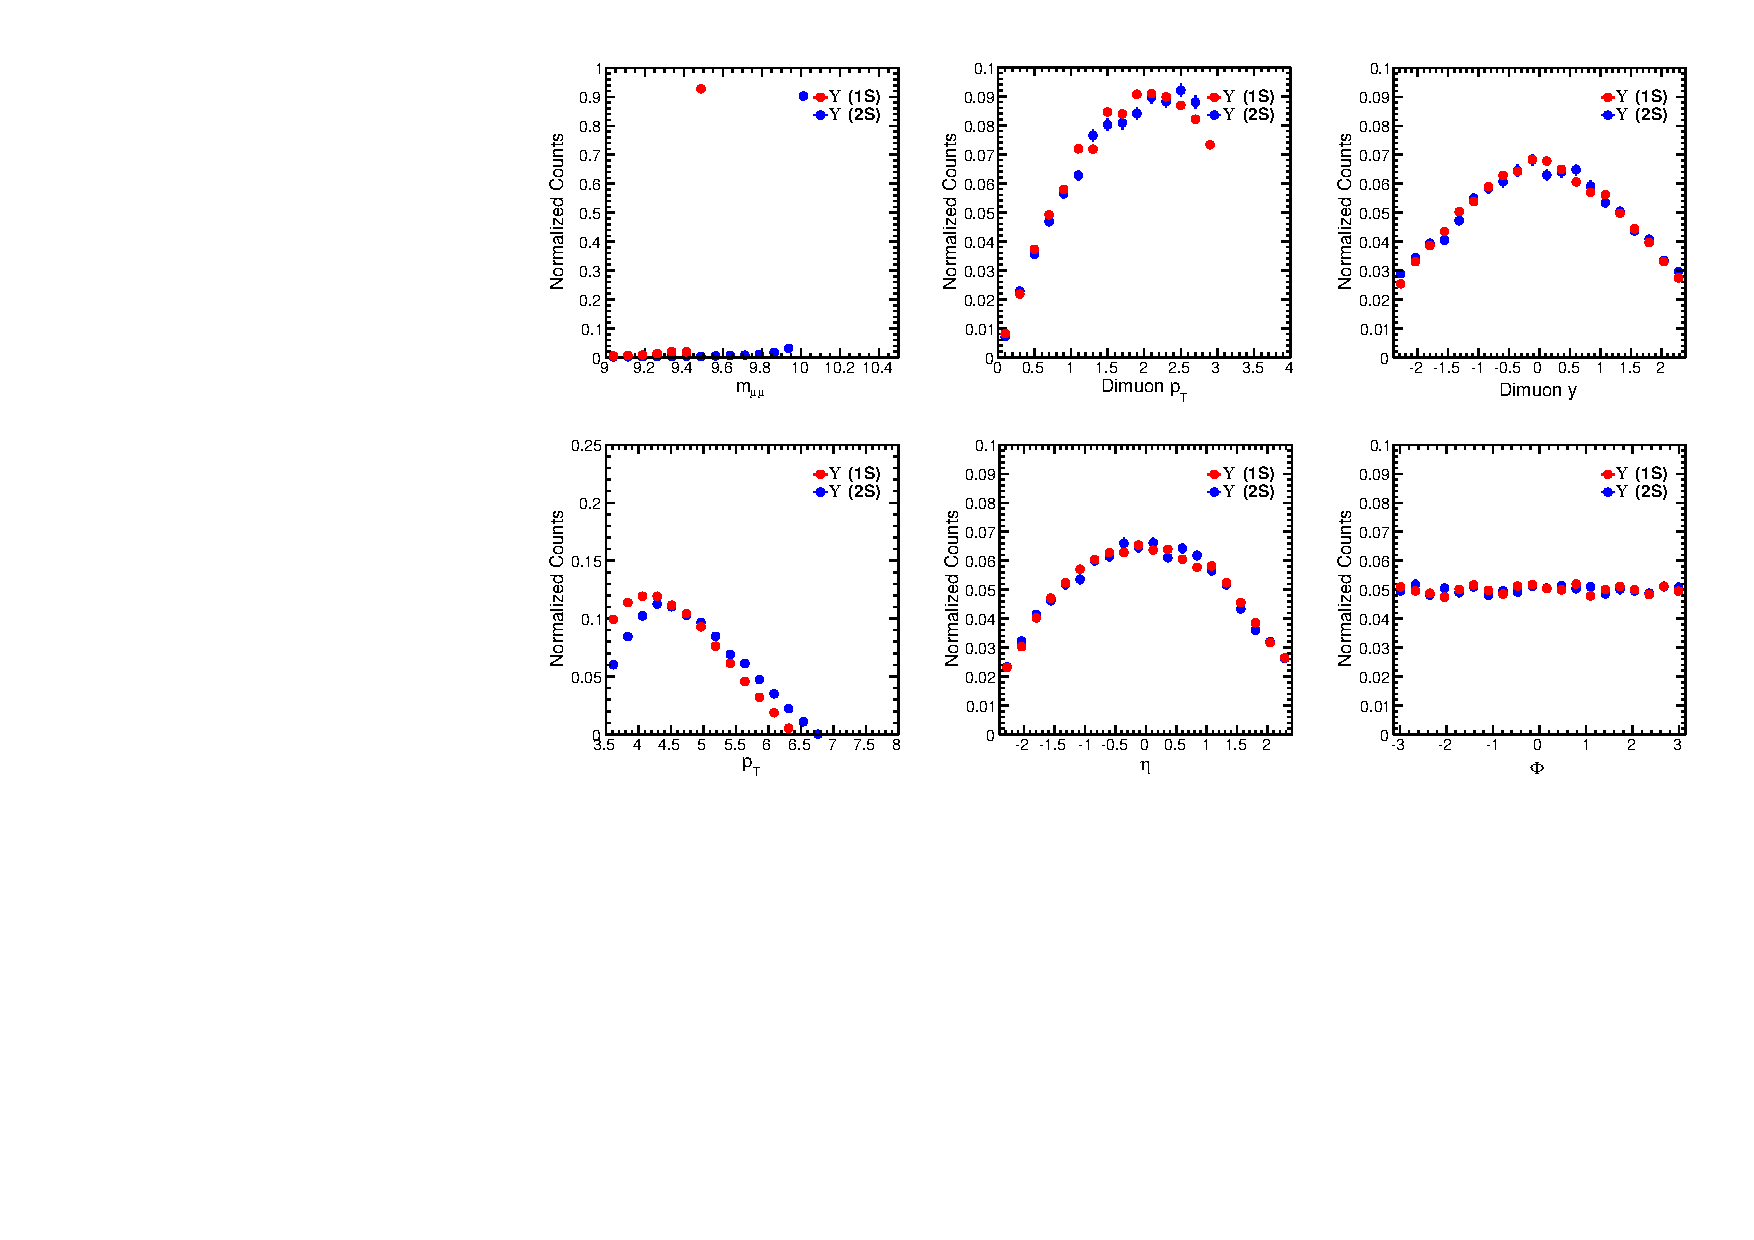
\includegraphics[angle=0,width=1.0\textwidth]{figures/efficiency/Plots_for_Upsilon_PbPb_3_and_a_half}\label{fig:muon_properties_PbPb_3_5}}\\
%    \caption{(top row) Normalized mass, $p_{T}$ and y distributions of the generated \PgUa and \PgUb in \PbPb events. (bottom row) Normalized $p_{T}$, $\eta$ and $\phi$ distributions for the individual muons.The muon kinematic requirement $\pt > 3.5\GeVc$ is applied. }
%    \label{fig:muon_properties_PbPb_3_5}
%  \end{center}
%\end{figure}
%
%\begin{figure}[h]
%  \begin{center}
    \subfigure[\pp MC simulation]{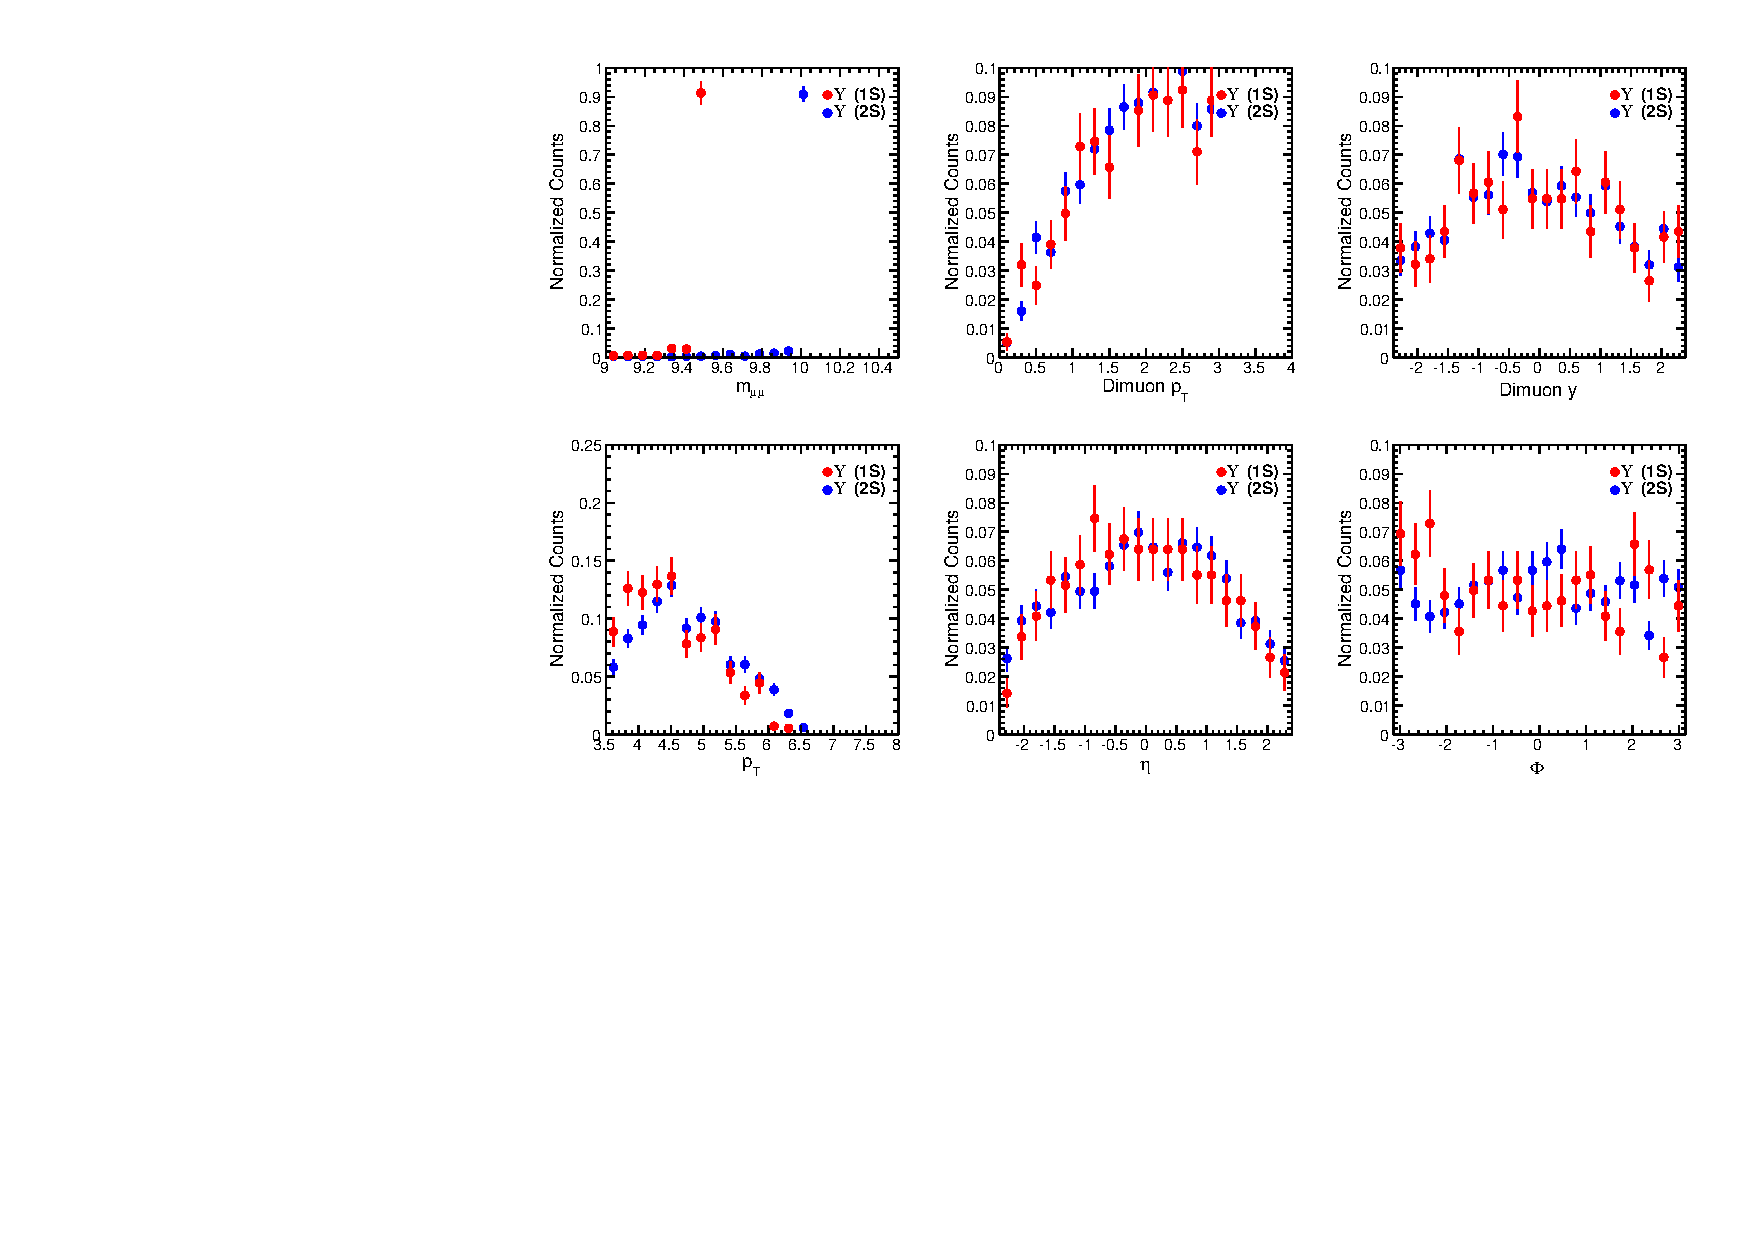
\includegraphics[angle=0,width=1.0\textwidth]{figures/efficiency/Plots_for_Upsilon_pp_3_and_a_half}\label{fig:muon_properties_pp_3_5}}
%    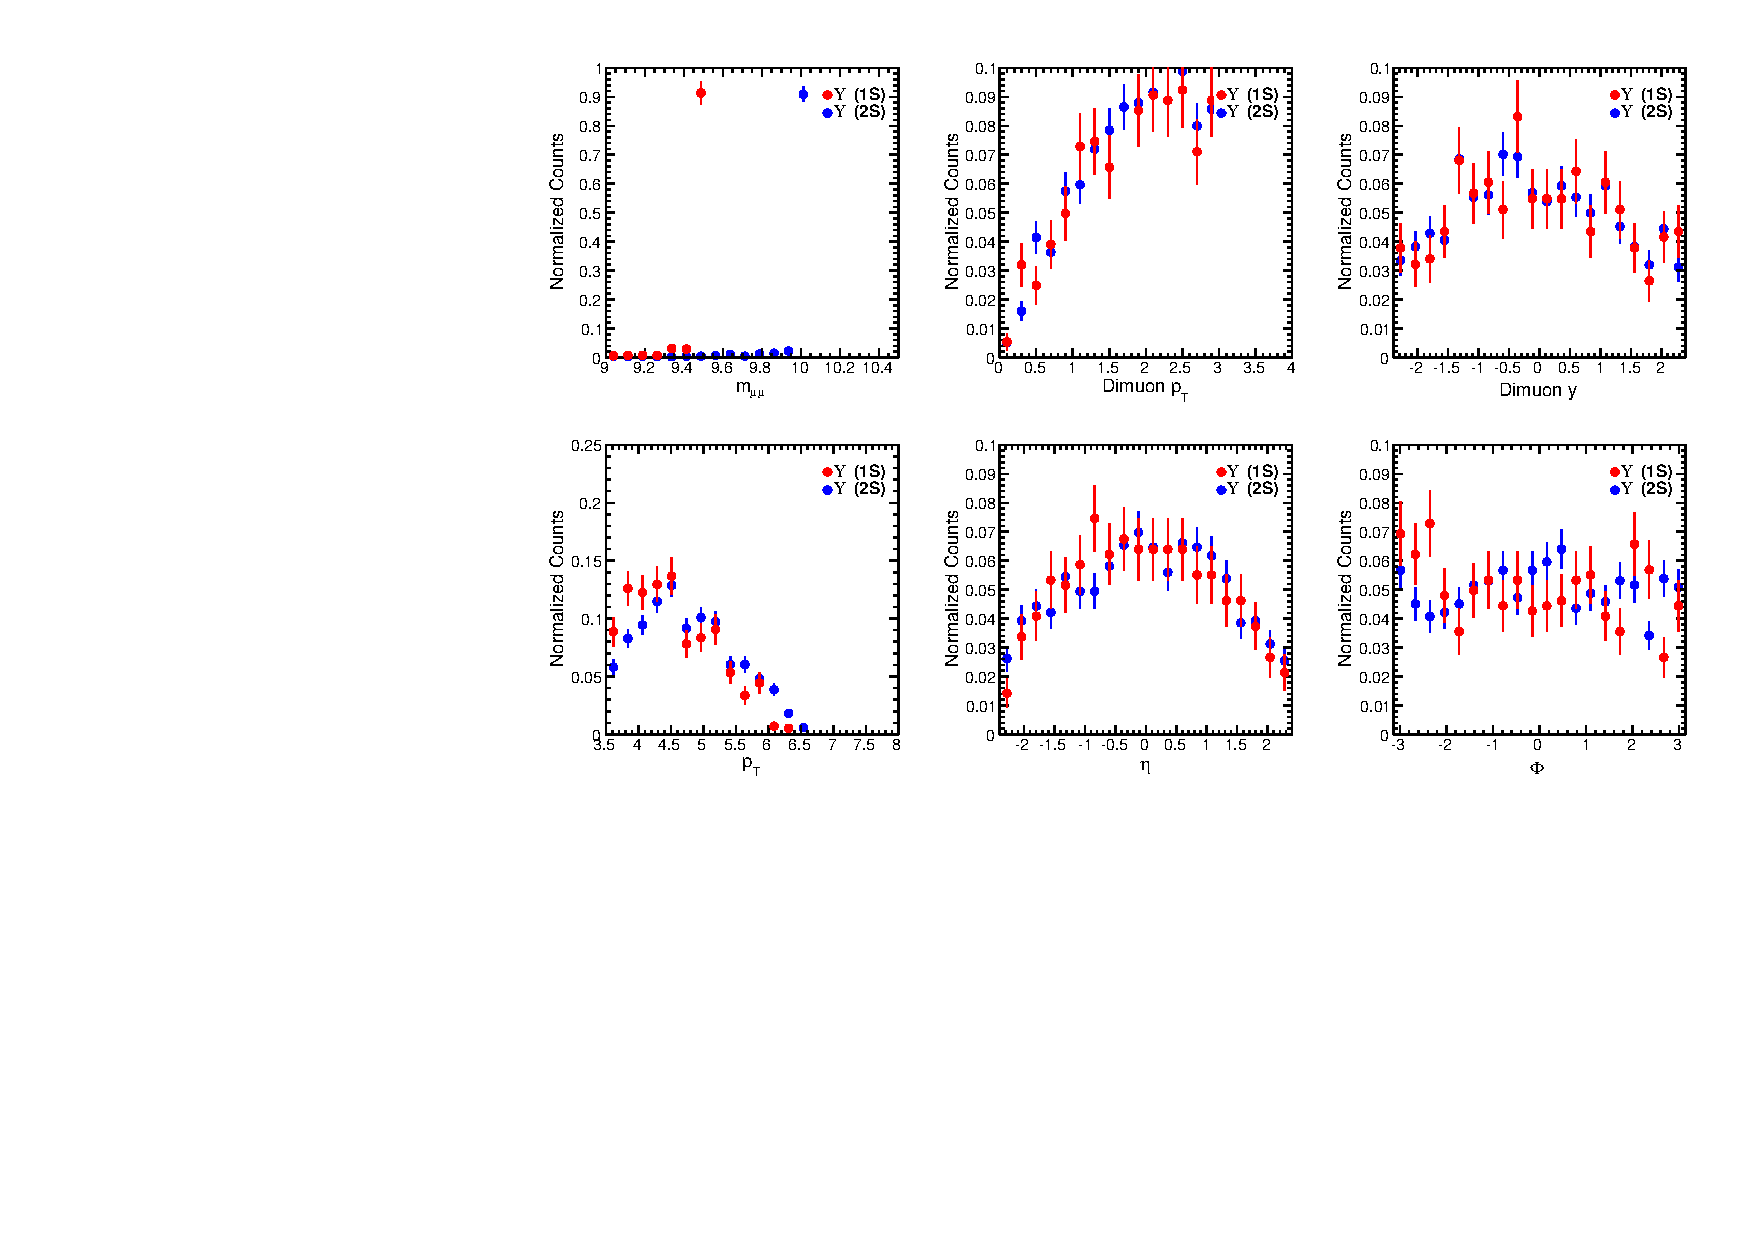
\includegraphics[angle=0,width=1.0\textwidth]{figures/efficiency/Plots_for_Upsilon_pp_3_and_a_half}\hspace{1em}
%    \caption{(top row) Normalized mass, $p_{T}$ and y distributions of the generated \PgUa and \PgUb in \pp events. (bottom row) Normalized $p_{T}$, $\eta$ and $\phi$ distributions for the individual muons.The muon kinematic requirement $\pt > 3.5\GeVc$ is applied. }
    \caption{Comparison of \PgUa and \PgUb kinematic distributions in \PbPb and \pp MC simulation: 
invariant mass, \pt and $y$ di-muon normalized distributions, and 
$\pt$, $\eta$ and $\phi$ single-muon normalized distributions.
The muon kinematic requirement $\pt > 3.5\GeVc$ is applied. 
}
    \label{fig:muon_properties_3_5}
  \end{center}
\end{figure}


